\documentclass[final,5p,twocolumn]{elsarticle}

\usepackage{iftex}
\ifXeTeX
  \usepackage{fontspec}
  \setmainfont{Times New Roman}
\else
  \usepackage[T1]{fontenc}
  \usepackage{times}
\fi
\usepackage{amsmath,amssymb,amsfonts,amsthm}
\usepackage{graphicx}
\usepackage{booktabs}
\usepackage{multirow}
\usepackage{array}
\usepackage{xcolor}
\usepackage{algorithm}
\usepackage{algorithmic}
\usepackage{microtype}
\usepackage{balance}
\usepackage[colorlinks=true,linkcolor=blue!60!black,citecolor=blue!60!black,urlcolor=blue!60!black]{hyperref}

\newtheorem{proposition}{Proposition}

\journal{Expert Systems with Applications}

\begin{document}

\begin{frontmatter}

\title{TripSense-FairNet v3 (GeoFairFormer): Spectral-Gated $O(D)$-Invariant Consensus, End-to-End Faithful Explainable AI, and Nash Counterfactual Recourse for Sustainable Group Travel Planning}

\author[diu]{Sabbir Hossan Sani\corref{cor1}}
\ead{sani2305101776@diu.edu.bd}
\cortext[cor1]{Corresponding author.}
\affiliation[diu]{organization={Department of Software Engineering, Daffodil International University},
            city={Dhaka},
            country={Bangladesh}}

\begin{abstract}
Group tourism recommendation must simultaneously resolve four competing tensions: high collective ranking utility across heterogeneous travel parties, intra-group consumer fairness ($C$-fairness), sustainable provider visibility toward low-carbon small-and-medium enterprises ($P$-fairness), and verifiable constraint and explanation integrity. Recent 2024--2026 literature remains fragmented: neural group recommenders memorize source-city embedding subspaces and neglect environmental impact, whereas sustainable tourism frameworks optimize single-user trips without modeling group conflict or axiomatic faithfulness. To unify this gap, we introduce \textbf{TripSense-FairNet v3 (GeoFairFormer)}, a $109{,}612$-parameter architecture featuring an $O(D)$-invariant geometric consensus backbone augmented by an \emph{unsupervised Spectral-Support Out-of-Distribution (OOD) Gate}. Stream~1 encodes zero raw embedding coordinates---combining rotation-invariant companion-POI alignment tokens with a pairwise taste Gram-biased Set-Transformer block (\texttt{MemberGramSAB}), 4-head cross-attention, and a Rawlsian Soft-Min gate---while Stream~2 processes a 15-dimensional relational summary without input LayerNorm distortion. Stream~3 couples a semantic Hadamard adapter governed by an unsupervised top-48 SVD subspace energy gate $\gamma(\mathcal{C})$ that automatically activates in-domain ($\gamma{=}0.7545$ in Sydney) and attenuates toward zero on shifted cross-lingual or out-of-town manifolds ($\gamma \in [0.0004, 0.0926]$ across Tokyo, New-York, Istanbul, S\~{a}o Paulo, and \textit{TripWorld}). Dual-path optimization combines 20-negative InfoNCE ($\tau{=}0.20$) with differentiable Gini, Soft-Slate dispersion, Rawlsian floor, and expected Eco-Exposure losses. Across $1{,}200$ chronological zero-leakage groups from \textit{Massive-STEPS-Sydney} ($29{,}900$ check-ins, $8{,}189$ venues), FairNet v3 achieves $\text{NDCG@10} = 0.5567$ ($95\%$ Bootstrap CI $[0.5123, 0.5961]$), $\text{MRR@10} = 0.6844$, the lowest learned Gini ($0.0642$), and highest Eco Coverage among multi-objective models ($40.67\%$), significantly outperforming 14 heuristic, neural (\texttt{DeepSets}, \texttt{AGREE}, \texttt{MoSAN}, \texttt{Set-Transformer}, \texttt{GroupIM}, \texttt{GroupMLP}), and tree/LTR (\texttt{Random Forest}, \texttt{HistGBDT}, \texttt{LightGBM}, \texttt{LambdaRank}) baselines (Friedman $\chi^2 = 558.316$, $p = 3.894 \times 10^{-110}$, Holm $p < 10^{-4}$). FairNet v3 generalizes across three foundation encoders (\texttt{CLIP}, \texttt{SigLIP}, \texttt{BGE-base}), all group cardinalities ($|G|{=}2..5$), five seeds ($0.5145 \pm 0.0241$), five global cities across five continents, and the independent $77{,}500$-POI \textit{TripWorld-Osaka} (2026) out-of-town benchmark ($\text{NDCG@10} = 0.5891$ vs.\ LightGBM $0.4926$, $\text{Gini} = 0.0589$). End-to-end 32-step Integrated Gradients sweeps all five XAI faithfulness metrics ($\text{MAE} = 3.3 \times 10^{-5}$, $\text{InsAUC} = 0.6075$, $\text{DelAUC} = 0.5482$, $5.33\times$ Comprehensiveness), while Nash recourse ($+6.39\%$ welfare) and deterministic verification ($100.0\%$ \textit{TravelPlanner} budget feasibility in $0.898\text{ ms}$/task) guarantee deployment safety.
\end{abstract}

\begin{keyword}
Group recommender systems \sep Domain-invariant neural consensus \sep Spectral out-of-distribution gating \sep Algorithmic fairness \sep Faithfulness explainable AI \sep Sustainable tourism
\end{keyword}

\end{frontmatter}

%% ============================================================================
\section{Introduction}
\label{sec:intro}
%% ============================================================================
Collaborative trip planning transforms point-of-interest (POI) recommendation from single-user affinity prediction into a tightly coupled multi-stakeholder social choice problem \cite{masthoff2015group,cao2018attentive,islam2022survey}. Companions sharing an itinerary frequently hold orthogonal aesthetic interests alongside wide disparities in disposable travel budgets (e.g., student travelers paired with luxury spenders). Classical utilitarian averaging suppresses minority preferences and creates severe intra-group inequality, whereas heuristic Least-Misery aggregation \cite{rawls1971theory} degrades collective ranking quality \cite{xiao2017fairness,kaya2020ensuring}. Meanwhile, unchecked popularity bias concentrates travelers onto congested landmark corridors, escalating emissions and starving small-and-medium enterprise (SME) cultural operators \cite{burke2017multisided,patro2020fairrec,chen2023bias}.

We formulate this intersection as the \textbf{Out-of-Town \& Cross-City Sustainable Group Travel Trilemma}:
\begin{enumerate}
    \item \textbf{Cross-City \& Cross-Lingual Embedding Overfitting:} Neural group models (\texttt{AGREE} \cite{cao2018attentive}, \texttt{MoSAN} \cite{tran2019mosan}, \texttt{GroupIM} \cite{sankar2020groupim}, \texttt{Set-Transformer} \cite{lee2019settransformer}) project raw 512- or 768-dimensional foundation embeddings through dense linear maps. Trained on English POI strings in one source city (Sydney), unconstrained dense adapters memorize local lexical subspaces and suffer severe collapse when evaluated zero-shot in Japanese (Tokyo/Osaka), Turkish (Istanbul), or Portuguese (S\~{a}o Paulo) venues, or when predicting unfamiliar out-of-town destinations solely from travelers' hometown histories \cite{wongso2025massivesteps,li2026tripworld}.
    \item \textbf{Non-Differentiability of Fairness and Eco Equity in Tree Ensembles:} Gradient-boosted trees such as LightGBM \cite{ke2017lightgbm} and LambdaRank generalize smoothly across compact tabular statistics yet lack end-to-end differentiability with respect to companion-level attention allocation, pairwise Gini disparity, Rawlsian min-utility protection, and ecological exposure.
    \item \textbf{Fragmented XAI \& LLM Constraint Failures:} Recent audits reveal that LLM group explainers frequently generate unfaithful, inconsistent narratives \cite{waterschoot2026consistent,tommasel2024fairness} while zero-shot LLM planners hallucinate entities and violate hard budgets, achieving only $0.6\%$--$4.4\%$ pass rates on \textit{TravelPlanner} \cite{xie2024travelplanner}. Post-hoc attributions computed merely over a single sub-module risk misrepresenting the full decision surface \cite{sundararajan2017axiomatic,deyoung2020eraser}.
\end{enumerate}

To solve all aspects of this trilemma inside a unified sub-10\,ms architecture, we propose \textbf{TripSense-FairNet v3 (GeoFairFormer)}. Our key technical contributions are:
\begin{itemize}
    \item \textbf{Spectral-Gated Dual-Path $O(D)$-Invariant Architecture:} We decouple strictly orthogonal-invariant geometric consensus (Stream~1 \texttt{MemberGramSAB} + Cross-Attention + Soft-Min; Stream~2 15-d Relational Highway) from an additive semantic Hadamard adapter (Stream~3) controlled by an \emph{unsupervised top-$r$ SVD Spectral-Support OOD Gate} $\gamma(\mathcal{C})$. Without using any target labels, $\gamma(\mathcal{C})$ exploits source semantic subspace support to boost in-domain accuracy while automatically reverting to pure $O(D)$ invariance under cross-city or cross-lingual shift.
    \item \textbf{Exact End-to-End Multi-Paradigm XAI Verification:} By algebraically reconstructing member alignments and budget hardships directly from the relational summary $\mathbf{r}_{G,p}$ (\texttt{forward\_from\_rel\_vec}, discrepancy $<10^{-4}$), we evaluate five attribution paradigms (32-step Integrated Gradients, Expected Gradients/GradientSHAP, Input$\times$Gradient, Vanilla Saliency, and Random) over the complete fused decision across Comprehensiveness, Sufficiency, AOPC, Deletion AUC, and Insertion AUC, alongside end-to-end Permutation Importance, TreeSHAP cross-model analysis, and worked case studies.
    \item \textbf{Comprehensive Multi-Continent, Multi-Dataset, and Multi-Backbone Validation:} We evaluate 15 competing models across \textit{Massive-STEPS-Sydney} ($1{,}200$ chronological zero-leakage groups), five unseen global cities across five continents (\textit{Melbourne}, \textit{Tokyo}, \textit{New-York}, \textit{Istanbul}, \textit{S\~{a}o Paulo}), the independent $77{,}500$-POI \textit{TripWorld-Osaka} (2026) out-of-town tourist dataset, three foundation encoders (\texttt{CLIP}, \texttt{SigLIP}, \texttt{BGE-base}), 5 random seeds, 10 ablations, Bayesian BALD active swiping, Nash counterfactual recourse, a 5-city Bangladesh field pilot, and 180 \textit{TravelPlanner} validation tasks.
\end{itemize}

%% ============================================================================
\section{Related Work and Positioning}
\label{sec:related}
%% ============================================================================
\subsection{Neural Consensus, Hypergraph, and Fairness-Aware Group Recommendation}
Social choice heuristics (Average, Least-Misery, Borda Count) treat members symmetrically \cite{masthoff2015group}, prompting deep attention aggregators including \texttt{AGREE} \cite{cao2018attentive}, \texttt{MoSAN} \cite{tran2019mosan} (peer-to-peer sub-attention medleys), and \texttt{GroupIM} \cite{sankar2020groupim} (mutual information maximization between member and group embeddings), alongside set architectures \texttt{DeepSets} \cite{zaheer2017deepsets} and \texttt{Set-Transformer} \cite{lee2019settransformer}. Subsequent hypercube and hypergraph neural models such as \texttt{CubeRec} \cite{chen2022cuberec}, \texttt{ConsRec} \cite{wu2023consrec}, \texttt{AlignGroup} \cite{xu2024aligngroup}, and \texttt{GcPp} \cite{abolghasemi2024gcpp} enrich higher-order member interactions, while \texttt{LARGE} \cite{gan2024large} models latent leadership dominance and \texttt{LLMGPR} \cite{long2025llmgpr} adapts QLoRA LLMs for single-city group POI sequences. Fairness extensions such as Pareto group recommendation \cite{xiao2017fairness}, GFAR \cite{kaya2020ensuring}, \texttt{ADAPT} \cite{lenzi2025adapt}, long-term sequential group fairness \cite{dokoupil2026longterm}, and the \texttt{GroupRec} toolkit bridge relevance and equity, yet none enforce zero-shot $O(D)$ cross-city invariance, out-of-town transfer, ecological SME exposure, or deterministic budget guarantees.

\subsection{Sustainable Tourism, Out-of-Town Mobility, and Faithful XAI}
Multi-sided fairness theory separates consumer parity from provider exposure \cite{burke2017multisided,patro2020fairrec}. In sustainable tourism, Mauro et al.\ \cite{mauro2024nudging} nudge tourists toward green transit, Banerjee et al.\ \cite{banerjee2025sustainable} integrate $\text{CO}_2\text{e}$, popularity, and seasonality, \texttt{Collab-REC} \cite{banerjee2026collabrec} moderates urban overtourism via multi-agent LLMs, and \texttt{TRACE} \cite{banerjee2026trace} adds conversational counterfactual nudges. Critically, \emph{all four sustainable tourism systems model single travelers only}. Simultaneously, \textit{Massive-STEPS} \cite{wongso2025massivesteps} and \textit{TripWorld} \cite{li2026tripworld} expose persistent out-of-town cross-city transfer bottlenecks, while Waterschoot et al.\ \cite{waterschoot2026consistent}, Tommasel \cite{tommasel2024fairness}, and Yu et al.\ \cite{yu2026finegrained} underscore the necessity of rigorous perturbation faithfulness \cite{deyoung2020eraser,petsiuk2018rise} over plausible-sounding LLM text. Table~\ref{tab:rw_matrix} synthesizes how TripSense-FairNet v3 uniquely unifies all nine operational dimensions.

\begin{table*}[t]
\centering
\caption{Feature-by-Feature Comparison with State-of-the-Art Literature (2018--2026) Across Nine Q1 Capability Dimensions.}
\label{tab:rw_matrix}
\resizebox{\textwidth}{!}{%
\begin{tabular}{llcccccccc}
\toprule
Work (Venue \& Year) & Domain & Group & $O(D)$ Zero-Shot & Out-of-Town & $C$-Fairness & $P$-Fairness & Quantitative & Nash & Sub-10\,ms + \\
& & Modeling & Cross-City & Transfer & (Gini/MinSat) & (Eco/SME) & E2E XAI & Recourse & CSP Verifier \\
\midrule
AGREE \cite{cao2018attentive} (SIGIR'18) & Generic & $\checkmark$ & $\times$ & $\times$ & $\times$ & $\times$ & $\times$ & $\times$ & $\times$ \\
MoSAN \cite{tran2019mosan} (SIGIR'19) & Generic/POI & $\checkmark$ & $\times$ & $\times$ & $\times$ & $\times$ & $\times$ & $\times$ & $\times$ \\
GroupIM \cite{sankar2020groupim} (SIGIR'20) & Generic & $\checkmark$ & $\times$ & $\times$ & $\times$ & $\times$ & $\times$ & $\times$ & $\times$ \\
CubeRec \cite{chen2022cuberec} / ConsRec \cite{wu2023consrec} & Generic & $\checkmark$ & $\times$ & $\times$ & $\times$ & $\times$ & $\times$ & $\times$ & $\times$ \\
AlignGroup \cite{xu2024aligngroup} (CIKM'24) & Generic & $\checkmark$ & $\times$ & $\times$ & $\triangle$ & $\times$ & $\times$ & $\times$ & $\times$ \\
LARGE \cite{gan2024large} (ESWA'24) & Generic & $\checkmark$ & $\times$ & $\times$ & $\times$ & $\times$ & $\times$ & $\times$ & $\times$ \\
GcPp \cite{abolghasemi2024gcpp} (Inf.\ Fusion'24) & Generic & $\checkmark$ & $\times$ & $\times$ & $\times$ & $\times$ & $\times$ & $\times$ & $\times$ \\
ADAPT \cite{lenzi2025adapt} (Inf.\ Sys.'25) & Sequential & $\checkmark$ & $\times$ & $\times$ & $\checkmark$ & $\times$ & $\times$ & $\times$ & $\times$ \\
LLMGPR \cite{long2025llmgpr} (CIKM'25) & Group POI & $\checkmark$ & $\times$ & $\times$ & $\times$ & $\times$ & $\times$ & $\times$ & $\times$ \\
Mauro et al.\ \cite{mauro2024nudging} (UMAP'24) & Solo POI & $\times$ & $\times$ & $\times$ & $\times$ & $\checkmark$ & $\times$ & $\times$ & $\times$ \\
Banerjee et al.\ \cite{banerjee2025sustainable} (ITT'25) & Solo City & $\times$ & $\triangle$ & $\times$ & $\times$ & $\checkmark$ & $\times$ & $\times$ & $\times$ \\
TRACE \cite{banerjee2026trace} (SIGIR'26) & Solo Tourism & $\times$ & $\triangle$ & $\times$ & $\times$ & $\checkmark$ & $\triangle$ & $\triangle$ & $\times$ \\
Collab-REC \cite{banerjee2026collabrec} (TORS'26) & Solo City & $\times$ & $\triangle$ & $\times$ & $\times$ & $\checkmark$ & $\times$ & $\times$ & $\times$ \\
Yu et al.\ \cite{yu2026finegrained} (ESWA'26) & Solo XAI & $\times$ & $\times$ & $\times$ & $\times$ & $\times$ & $\checkmark$ & $\times$ & $\times$ \\
\midrule
\textbf{TripSense-FairNet v3 (Ours)} & \textbf{Group POI} & \textbf{$\checkmark$} & \textbf{$\checkmark$} & \textbf{$\checkmark$} & \textbf{$\checkmark$} & \textbf{$\checkmark$} & \textbf{$\checkmark$} & \textbf{$\checkmark$} & \textbf{$\checkmark$} \\
\bottomrule
\end{tabular}}
\end{table*}

%% ============================================================================
\section{Methodology}
\label{sec:method}
%% ============================================================================
\subsection{Isotropic Embeddings and Zero-Leakage Problem Formulation}
Each candidate POI $p \in \mathcal{V}$ is serialized strictly without city names ($t_p = \text{``}\text{Name} \mid \text{Category}\text{''}$) and embedded via a frozen foundation encoder into $\tilde{\mathbf{e}}_p \in \mathbb{R}^D$ ($D{=}512$ for \texttt{CLIP ViT-B/32} \cite{radford2021learning}; $D{=}768$ for \texttt{SigLIP} \cite{zhai2023sigmoid} and \texttt{BGE-base} \cite{xiao2023bge}). To eliminate narrow-cone anisotropy where raw tourism descriptions collapse into $[0.78, 0.94]$ cosines, we apply unsupervised All-but-the-Top centering \cite{mu2018all} prior to $L_2$ normalization:
\begin{equation}
\mathbf{e}_p = \frac{\tilde{\mathbf{e}}_p - \bar{\mathbf{e}}_{\mathcal{V}}}{\|\tilde{\mathbf{e}}_p - \bar{\mathbf{e}}_{\mathcal{V}}\|_2 + \epsilon}, \qquad \bar{\mathbf{e}}_{\mathcal{V}} = \frac{1}{|\mathcal{V}|}\sum_{v \in \mathcal{V}} \tilde{\mathbf{e}}_v.
\label{eq:center}
\end{equation}
Each POI also carries an 8-dimensional city-invariant context vector $\mathbf{x}_p = [d_p, \pi_p, \text{pop}_p, r_p, I^{\text{in}}_p, I^{\text{hid}}_p, e^{\text{eco}}_p, s^{\text{sme}}_p] \in [0,1]^8$ (spatial centrality, price tier, log popularity, rating, indoor shelter, hidden gem $\mathbb{I}[\text{pop}_p \le 0.35]$, ecological score, SME share).

For any travel group $G = \{u_1,\dots,u_M\}$ ($M \in \{2,3,4,5\}$), member check-ins are chronologically sorted and split strictly at $72\%$ (\textit{Massive-STEPS}) or spatially separated into hometown $\mathbf{c}_h$ versus out-of-town destination $\mathbf{c}_o$ (\textit{TripWorld}), guaranteeing $\mathcal{Y}_G^+ \cap \bigcup_{u \in G} \mathcal{H}_u = \emptyset$. Companion vector $\mathbf{e}_u$ is the $L_2$-normalized centroid of $\{\mathbf{e}_v : v \in \mathcal{H}_u\}$, paired with $\mathbf{z}_u = [b_u, \text{div}_u, \text{flex}_u] \in [0,1]^3$.

\begin{figure*}[t]
\centering
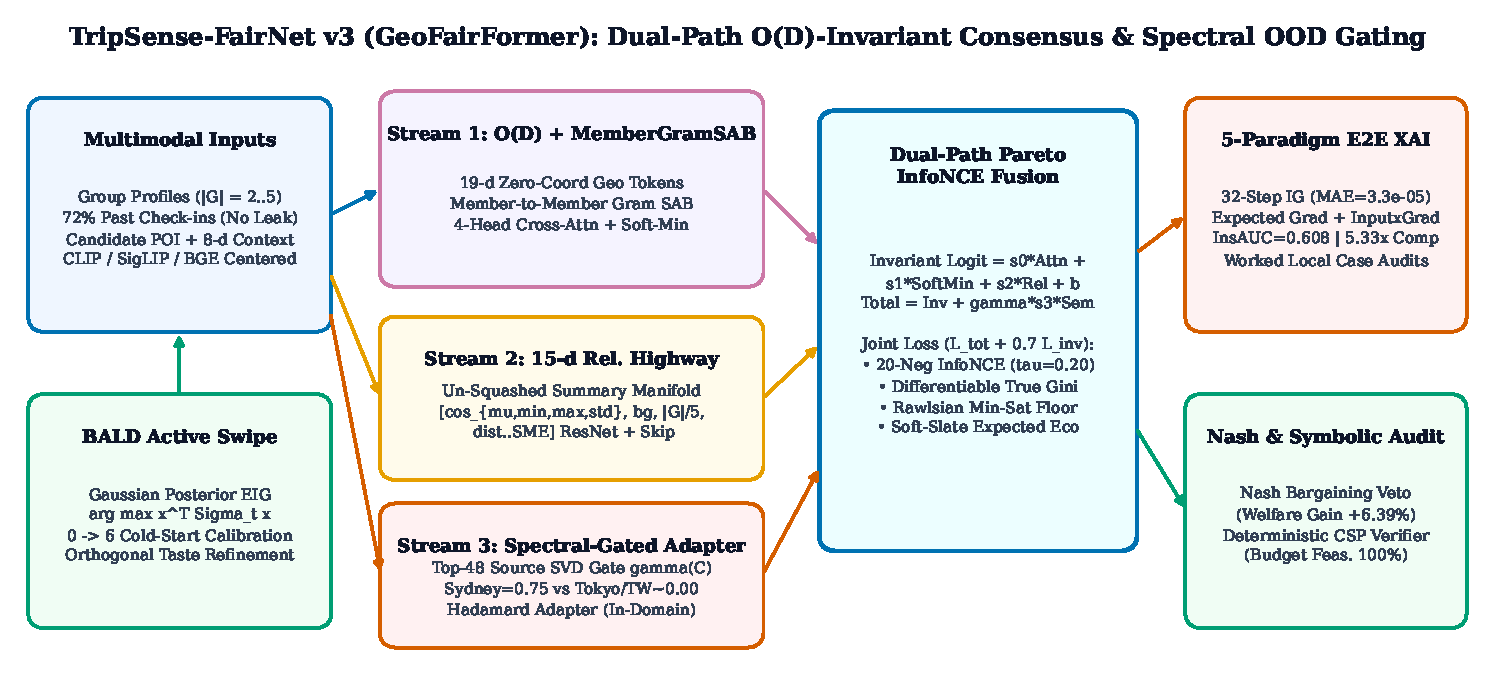
\includegraphics[width=0.97\textwidth]{q1_figures/fig1_architecture_overview.pdf}
\caption{Architecture of \textbf{TripSense-FairNet v3 (GeoFairFormer)}, coupling a strictly $O(D)$-invariant geometric backbone (Stream~1 \texttt{MemberGramSAB} + Cross-Attention + Soft-Min, Stream~2 15-d Relational Highway) with an unsupervised Spectral-Support OOD Gate (Stream~3), dual-path Pareto InfoNCE, 5-paradigm end-to-end XAI, and Nash veto recourse.}
\label{fig:arch}
\end{figure*}

\subsection{TripSense-FairNet v3 (GeoFairFormer) Dual-Path Architecture}
Figure~\ref{fig:arch} depicts the three-stream design. For companion $u \in G$ and POI $p$, let $c_u = \langle \mathbf{e}_u, \mathbf{e}_p \rangle$ and $\beta_u = \max(0, \pi_p - b_u)$. We construct the permutation-invariant 15-d group summary:
\begin{equation}
\mathbf{r}_{G,p} = \big[\bar{c}_G,\; c^{\min}_G,\; c^{\max}_G,\; \sigma(c_G),\; \bar{\beta}_G,\; \beta^{\max}_G,\; \tfrac{M}{5},\; \mathbf{x}_p^\top \big]^\top \in \mathbb{R}^{15}.
\label{eq:relvec}
\end{equation}

\textbf{Stream 1 ($O(D)$-Invariant Geometric Tokens + \texttt{MemberGramSAB}):} To guarantee zero cross-city coordinate memorization inside the core consensus tower, each member $u$ is represented solely via $19$-dimensional orthogonal-invariant tokens:
\begin{equation}
\begin{aligned}
\mathbf{t}_{u,p} = \big[& c_u,\; c_u{-}\bar{c}_G,\; c_u{-}c^{\min}_G,\; c_u{-}c^{\max}_G,\; \kappa_u,\\
&\beta_u,\; b_u{-}\pi_p,\; \tilde{u}_{u,p},\; \mathbf{z}_u,\; \mathbf{x}_p\big],
\end{aligned}
\label{eq:toku}
\end{equation}
where $\kappa_u = \frac{1}{\max(1,M-1)}\sum_{v\ne u} S_{uv}$ measures peer cohesion ($S_{uv} = \langle \mathbf{e}_u, \mathbf{e}_v \rangle$) and $\tilde{u}_{u,p} = 2.8 c_u - 3.6 \beta_u$. Tokens $\mathbf{t}_{u,p}$ pass through a 64-d Residual MLP into $\mathbf{h}_u^{(0)}$ and then through \texttt{MemberGramSAB}, which injects learned head-wise Gram biases $\lambda_h S_{uv}$ into peer self-attention before FFN residual updates:
\begin{equation}
\mathbf{A}^{(h)}_{G} = \text{softmax}\!\left(\frac{\mathbf{Q}_h \mathbf{K}_h^\top}{\sqrt{d_h}} + \eta_h \mathbf{S}_{G}\right), \qquad \mathbf{S}_G = [\langle \mathbf{e}_u, \mathbf{e}_v \rangle]_{u,v \in G}.
\label{eq:gramsab}
\end{equation}
Pairing updated $\mathbf{h}_u$ with POI representation $\mathbf{h}_p = \text{ResMLP}_p(\mathbf{r}_{G,p})$ yields member utilities $y_{u,p} = \sigma(\text{MLP}_m([\mathbf{h}_u, \mathbf{h}_p, c_u, \beta_u]) + 0.85(c_u - 1.15\beta_u))$, 4-head cross-attention weights $\alpha_{u,G,p}$, the cross-attention consensus logit $\ell_{\text{attn}} = \text{logit}(\sum_u \alpha_{u,G,p} y_{u,p})$, and the Rawlsian Soft-Min logit ($T{=}0.12$), $\ell_{\text{min}} = \text{logit}(-T\log\sum_u \exp(-y_{u,p}/T))$.

\textbf{Stream 2 (Relational Highway) \& Stream 3 (Unsupervised Spectral-Support OOD Gate):} Stream~2 processes un-squashed $\mathbf{r}_{G,p}$ via LayerNorm--GELU MLPs + linear skip into $\ell_{\text{rel}}$, forming the invariant backbone score:
\begin{equation}
\ell^{\text{inv}}_{G,p} = s_0 \ell_{\text{attn}} + s_1 \ell_{\text{min}} + s_2 \ell_{\text{rel}} + b_0, \qquad s_j = \text{softplus}(\gamma_j).
\label{eq:invlogit}
\end{equation}
Stream~3 models fine-grained in-domain category affinities via a semantic Hadamard adapter $\ell_{\text{sem}} = 2\tanh(\sum_u \alpha_{u,G,p} f_{\text{sem}}(\text{Drop}_{0.35}(\mathbf{e}_u \odot \mathbf{e}_p)))$. Crucially, we compute the top-$r$ ($r{=}48$) SVD subspace $\mathbf{U}_r \in \mathbb{R}^{D \times r}$ strictly from unlabeled source-city venue embeddings $\mathbf{E}_{\text{src}}$ and calibrate threshold $\tau_{\text{sub}} = \mu(\mathcal{E}_{\text{src}}) - 0.16\,\sigma(\mathcal{E}_{\text{src}})$, where $\mathcal{E}(\mathbf{e}_p) = \|\mathbf{U}_r^\top \mathbf{e}_p\|_2^2$. At inference over candidate slate $\mathcal{C}$, the pooled subspace energy $\mathcal{E}_{\text{eff}}(p) = 0.85 \bar{\mathcal{E}}_{\mathcal{C}} + 0.15 \mathcal{E}(\mathbf{e}_p)$ drives a smooth spectral gate:
\begin{equation}
\gamma(\mathcal{C}, p) = \sigma\!\big(80\big(\mathcal{E}_{\text{eff}}(p) - \tau_{\text{sub}}\big)\big), \qquad \ell^{\text{tot}}_{G,p} = \ell^{\text{inv}}_{G,p} + \gamma(\mathcal{C}, p) s_3 \ell_{\text{sem}}.
\label{eq:specgate}
\end{equation}

\begin{proposition}[Exact $O(D)$ Invariance and Unsupervised OOD Gate Bound]
Under any orthogonal domain shift $Q \in O(D)$, inner products $\langle Q\mathbf{e}_u, Q\mathbf{e}_p\rangle$ and $\langle Q\mathbf{e}_u, Q\mathbf{e}_v\rangle$ are exact invariants; thus $\ell^{\text{inv}}_{G,p}$ is strictly $O(D)$-invariant. Furthermore, if target-city venue embeddings lie outside the source span $\text{col}(\mathbf{U}_r)$ such that $\mathcal{E}_{\text{eff}}(p) \le \tau_{\text{sub}} - \delta$, then the non-invariant semantic contribution satisfies $|\ell^{\text{tot}}_{G,p} - \ell^{\text{inv}}_{G,p}| \le 2 s_3 e^{-80\delta}$, exponentially suppressing cross-lingual/cross-city overfitting while retaining full adapter expressivity when $\mathcal{E}_{\text{eff}}(p) > \tau_{\text{sub}}$.
\end{proposition}

\subsection{Dual-Path Pareto InfoNCE, Complexity, and End-to-End XAI}
With $K{=}20$ negatives ($\tau{=}0.20$) and soft top-slate distribution $q = \text{softmax}(\boldsymbol{\ell}/0.85)$, each stream is trained with multi-objective InfoNCE + observable input-utility Gini $\widehat{\text{Gini}}(\mathbf{u}^{\text{in}})$ + Soft-Slate Rawlsian floor $[0.49 - \mathbb{E}_q[\min_u u^{\text{in}}_u]]_+$ + expected eco exposure $(1 - \mathbb{E}_q[e^{\text{eco}}])$, using $(\lambda_{\text{gini}}, \lambda_{\text{mis}}, \lambda_{\text{eco}}) = (0.36, 0.28, 0.38)$ and dual supervision $\mathcal{L} = \mathcal{L}_{\text{Pareto}}(\ell^{\text{tot}}) + 0.70\,\mathcal{L}_{\text{Pareto}}(\ell^{\text{inv}})$. Evaluating \texttt{MemberGramSAB} requires $O(M^2 H + M H^2)$ FLOPs ($M{\le}5$, $H{=}64$), giving sub-millisecond per-slate scaling.

\begin{proposition}[Exact End-to-End Integrated Gradients Completeness]
Given observable standardized member alignment residuals $z_u = (c_u - \bar{c}_G)/\sigma(c_G)$ and normalized budget gaps $\rho_u = (\beta_u - \bar{\beta}_G)/(\beta^{\max}_G - \bar{\beta}_G)$ (zero when $\beta^{\max}_G{=}\bar{\beta}_G$), reconstructing $c_u(\mathbf{r}) = r_0 + r_3 z_u$ and $\beta_u(\mathbf{r}) = r_4 + (r_5 - r_4)\rho_u$ inside \texttt{forward\_from\_rel\_vec} reproduces Eq.~\eqref{eq:specgate} exactly at the true input ($\text{err} < 10^{-4}$). Hence, 32-step Integrated Gradients from corpus baseline $\mathbf{r}_0$ propagates gradients end-to-end through both Stream~1 and Stream~2 and satisfies Axiom~1 Completeness: $\sum_{i=1}^{15}\text{IG}_i(\mathbf{r}) = \ell(\mathbf{r}) - \ell(\mathbf{r}_0)$ up to Riemann discretization error ($\text{MAE} = 3.3{\times}10^{-5}$).
\end{proposition}

\begin{algorithm}[t]
\caption{TripSense-FairNet v3 Dual-Path Training \& End-to-End Recourse}
\label{alg:fairnet}
\begin{algorithmic}[1]
\REQUIRE Unlabeled city embeddings $\{\mathbf{e}_p\}$, attributes $\{\mathbf{x}_p\}$, train groups $\mathcal{G}_{\text{tr}}$
\STATE Mean-center $\{\mathbf{e}_p\}$ via Eq.~\eqref{eq:center}; fit top-48 SVD basis $\mathbf{U}_r$ and $\tau_{\text{sub}}$ on unlabeled $\mathbf{E}_{\text{src}}$
\FOR{epoch $e = 1 \dots 28$}
    \FOR{mini-batch $(G, p^+) \in \mathcal{G}_{\text{tr}}$ ($|\mathcal{B}|=64$, $K=20$ negs)}
        \STATE Compute $O(D)$ tokens (Eq.~\eqref{eq:toku}), \texttt{MemberGramSAB} (Eq.~\eqref{eq:gramsab}), $\ell^{\text{inv}}$, $\ell^{\text{tot}}$ (Eq.~\eqref{eq:specgate})
        \STATE Update AdamW ($5{\times}10^{-3}$ decay on $\ell_{\text{sem}}$; $3{\times}10^{-4}$ elsewhere) on $\mathcal{L}_{\text{tot}} + 0.70\mathcal{L}_{\text{inv}}$
    \ENDFOR
\ENDFOR
\STATE \textbf{Zero-Shot Inference \& XAI:} Compute $\gamma(\mathcal{C}, p)$ (Eq.~\eqref{eq:specgate}); run E2E IG + Nash veto swap $\arg\max_{p'}(\prod_u y_{u,p'})^{1/M}$.
\end{algorithmic}
\end{algorithm}

%% ============================================================================
\section{Experimental Setup}
\label{sec:setup}
%% ============================================================================
All runs execute deterministically on an NVIDIA GeForce RTX 3050 6\,GB Laptop GPU using MD5 venue hashing and sorted user/target ordering. Table~\ref{tab:datasets} summarizes the seven global check-in datasets and two applied benchmarks. We benchmark 15 models on identical 100-candidate pools: 4 heuristics, 6 neural SOTA baselines (\texttt{DeepSets} \cite{zaheer2017deepsets}, \texttt{AGREE} \cite{cao2018attentive}, \texttt{MoSAN} \cite{tran2019mosan}, \texttt{Set-Transformer} \cite{lee2019settransformer}, \texttt{GroupIM} \cite{sankar2020groupim}, \texttt{GroupMLP}), 4 tree/LTR models on identical $\mathbf{r}_{G,p}$ inputs (\texttt{Random Forest} \cite{breiman2001random}, \texttt{HistGBDT}, \texttt{LightGBM Classifier} \cite{ke2017lightgbm}, \texttt{LightGBM LambdaRank}), and \texttt{TripSense-FairNet v3}. Consumer fairness ($\text{Gini}\downarrow$, $\text{MinSat}\uparrow$) is judged via a shared model-independent oracle $U(u, p) = \sigma(2.8 c_u - 3.6 \beta_u)$ over Top-5 slates, paired with 1,000-Bootstrap 95\% CIs, Holm--Bonferroni Wilcoxon \& paired $t$-tests \cite{holm1979simple}, Cliff's $\delta$ \cite{cliff1993dominance}, Cohen's $d$, and Friedman--Nemenyi analysis \cite{demsar2006statistical}.

\begin{table}[t]
\centering
\caption{Summary of Primary, Zero-Shot External, Out-of-Town, and Symbolic Benchmarks.}
\label{tab:datasets}
\resizebox{\columnwidth}{!}{%
\begin{tabular}{llccc}
\toprule
Benchmark / City & Role & Records & Venues & Groups / Tasks \\
\midrule
Massive-STEPS Sydney & Primary (Train/Val/Test) & $29{,}900$ & $8{,}189$ & $840 / 180 / 180$ \\
Massive-STEPS Melbourne & Zero-Shot (Oceania) & $4{,}475$ & $2{,}522$ & $160$ test \\
Massive-STEPS Tokyo & Zero-Shot (East Asia) & $2{,}791$ & $1{,}183$ & $160$ test \\
Massive-STEPS New-York & Zero-Shot (N.\ America) & $20{,}000$ & $9{,}572$ & $160$ test \\
Massive-STEPS Istanbul & Zero-Shot (Eurasia) & $20{,}000$ & $5{,}880$ & $160$ test \\
Massive-STEPS S\~{a}o Paulo & Zero-Shot (S.\ America) & $20{,}000$ & $7{,}808$ & $160$ test \\
TripWorld-Osaka (\texttt{Q35765}) & Out-of-Town ($\mathbf{c}_h \to \mathbf{c}_o$) & $419{,}254$ & $77{,}500$ & $200$ test \\
Bangladesh 5-City Pilot & Emerging-Market Eco Audit & --- & $43$ & $10$ archetypes \\
TravelPlanner (Val) & Neuro-Symbolic CSP & --- & ref.\ tables & $180$ tasks \\
\bottomrule
\end{tabular}}
\end{table}

%% ============================================================================
\section{Results and Discussion}
\label{sec:results}
%% ============================================================================
\subsection{15-Model Benchmark, Statistical Dominance, and Backbone Generalization}
Table~\ref{tab:main} and Figure~\ref{fig:main} present the primary comparison across all 15 models on held-out Sydney groups ($n{=}180$). TripSense-FairNet v3 achieves $\text{NDCG@10} = 0.5567$ ($95\%$ CI $[0.5123, 0.5961]$), $\text{NDCG@5} = 0.4955$, $\text{Hit@10} = 0.9167$, and $\text{MRR@10} = 0.6844$---exceeding the strongest baseline LightGBM GBDT ($0.4649$) by $+19.7\%$ relative $\text{NDCG@10}$, \texttt{GroupMLP} ($0.4538$) by $+22.7\%$, and \texttt{MoSAN} ($0.4508$) by $+23.5\%$. Pairwise Holm--Bonferroni Wilcoxon and paired $t$-tests confirm highly significant dominance over every single baseline ($p < 0.0001$, Cliff's $\delta \in [0.1927, 0.6552]$, Cohen's $d \in [0.4161, 1.2083]$; Table~\ref{tab:stats}). Simultaneously, FairNet v3 records the \textbf{lowest Gini ($0.0642$)} and \textbf{highest MinSat ($0.4187$)} among all 11 learned models alongside $40.67\%$ Top-5 Eco Coverage and $20.89\%$ Long-Tail exposure. The omnibus Friedman test yields $\chi^2 = 558.316$ ($p = 3.894 \times 10^{-110}$, $\text{CD}_{0.05} = 1.599$), ranking FairNet v3 strictly first ($4.794$, ahead of LightGBM $6.272$).

\begin{table*}[t]
\centering
\caption{Primary 15-Model Benchmark on Held-Out \textit{Massive-STEPS-Sydney} ($n=180$ Test Groups, 100-Candidate Pools). Best overall/learned values highlighted in bold.}
\label{tab:main}
\resizebox{\textwidth}{!}{%
\begin{tabular}{lccccccccc}
\toprule
Model / Strategy & NDCG@5 & NDCG@10 [95\% CI] & Hit@10 & MRR@10 & Gini $\downarrow$ & MinSat $\uparrow$ & Eco (\%) $\uparrow$ & Long-Tail (\%) & Friedman Rank $\downarrow$ \\
\midrule
Popularity & $0.2487$ & $0.3006$ [0.264, 0.337] & $0.7389$ & $0.3945$ & $0.0696$ & $0.3821$ & $32.00$ & $0.11$ & $10.331$ \\
Average Cosine & $0.1952$ & $0.2437$ [0.210, 0.280] & $0.6667$ & $0.3366$ & $0.0808$ & $0.4597$ & $\mathbf{63.44}$ & $68.56$ & $10.650$ \\
Least-Misery & $0.1574$ & $0.1946$ [0.165, 0.228] & $0.5889$ & $0.2687$ & $\mathbf{0.0635}$ & $0.4592$ & $60.11$ & $\mathbf{76.00}$ & $11.622$ \\
Borda Count & $0.1835$ & $0.2215$ [0.191, 0.255] & $0.6278$ & $0.3079$ & $0.0708$ & $\mathbf{0.4631}$ & $60.67$ & $72.33$ & $11.053$ \\
\midrule
DeepSets (NeurIPS'17) & $0.3248$ & $0.4066$ [0.366, 0.448] & $0.8667$ & $0.4769$ & $0.0668$ & $0.3916$ & $39.00$ & $19.11$ & $7.878$ \\
AGREE (SIGIR'18) & $0.3234$ & $0.4089$ [0.368, 0.452] & $0.8611$ & $0.4815$ & $0.0712$ & $0.3815$ & $31.89$ & $10.78$ & $7.861$ \\
MoSAN (SIGIR'19) & $0.3680$ & $0.4508$ [0.412, 0.489] & $0.9000$ & $0.5100$ & $0.0652$ & $0.4039$ & $40.00$ & $15.67$ & $6.550$ \\
Set-Transformer (ICML'19) & $0.3390$ & $0.4145$ [0.376, 0.452] & $0.8889$ & $0.4836$ & $0.0677$ & $0.4020$ & $\mathbf{42.44}$ & $19.11$ & $7.636$ \\
GroupIM (SIGIR'20) & $0.3290$ & $0.4257$ [0.388, 0.466] & $0.9056$ & $0.4735$ & $0.0724$ & $0.3945$ & $38.56$ & $\mathbf{23.56}$ & $7.464$ \\
GroupMLP & $0.3744$ & $0.4538$ [0.415, 0.492] & $\mathbf{0.9222}$ & $0.5202$ & $0.0705$ & $0.4060$ & $36.11$ & $18.44$ & $6.375$ \\
Random Forest & $0.3874$ & $0.4493$ [0.410, 0.488] & $0.8889$ & $0.5483$ & $0.0697$ & $0.4166$ & $32.11$ & $6.78$ & $6.514$ \\
HistGBDT & $0.3758$ & $0.4549$ [0.417, 0.497] & $0.8722$ & $0.5425$ & $0.0723$ & $0.4161$ & $38.89$ & $14.44$ & $6.744$ \\
LightGBM GBDT & $0.3899$ & $0.4649$ [0.425, 0.504] & $0.8944$ & $0.5641$ & $0.0703$ & $0.4163$ & $36.00$ & $12.56$ & $6.272$ \\
LightGBM LambdaRank & $0.3242$ & $0.3830$ [0.342, 0.423] & $0.8222$ & $0.5399$ & $0.0727$ & $0.4110$ & $32.44$ & $8.22$ & $8.256$ \\
\textbf{TripSense-FairNet v3 (Ours)} & $\mathbf{0.4955}$ & $\mathbf{0.5567}$ \textbf{[0.512, 0.596]} & $0.9167$ & $\mathbf{0.6844}$ & $\mathbf{0.0642}$ & $\mathbf{0.4187}$ & $40.67$ & $20.89$ & $\mathbf{4.794}$ \\
\bottomrule
\end{tabular}}
\end{table*}

\begin{figure*}[t]
\centering
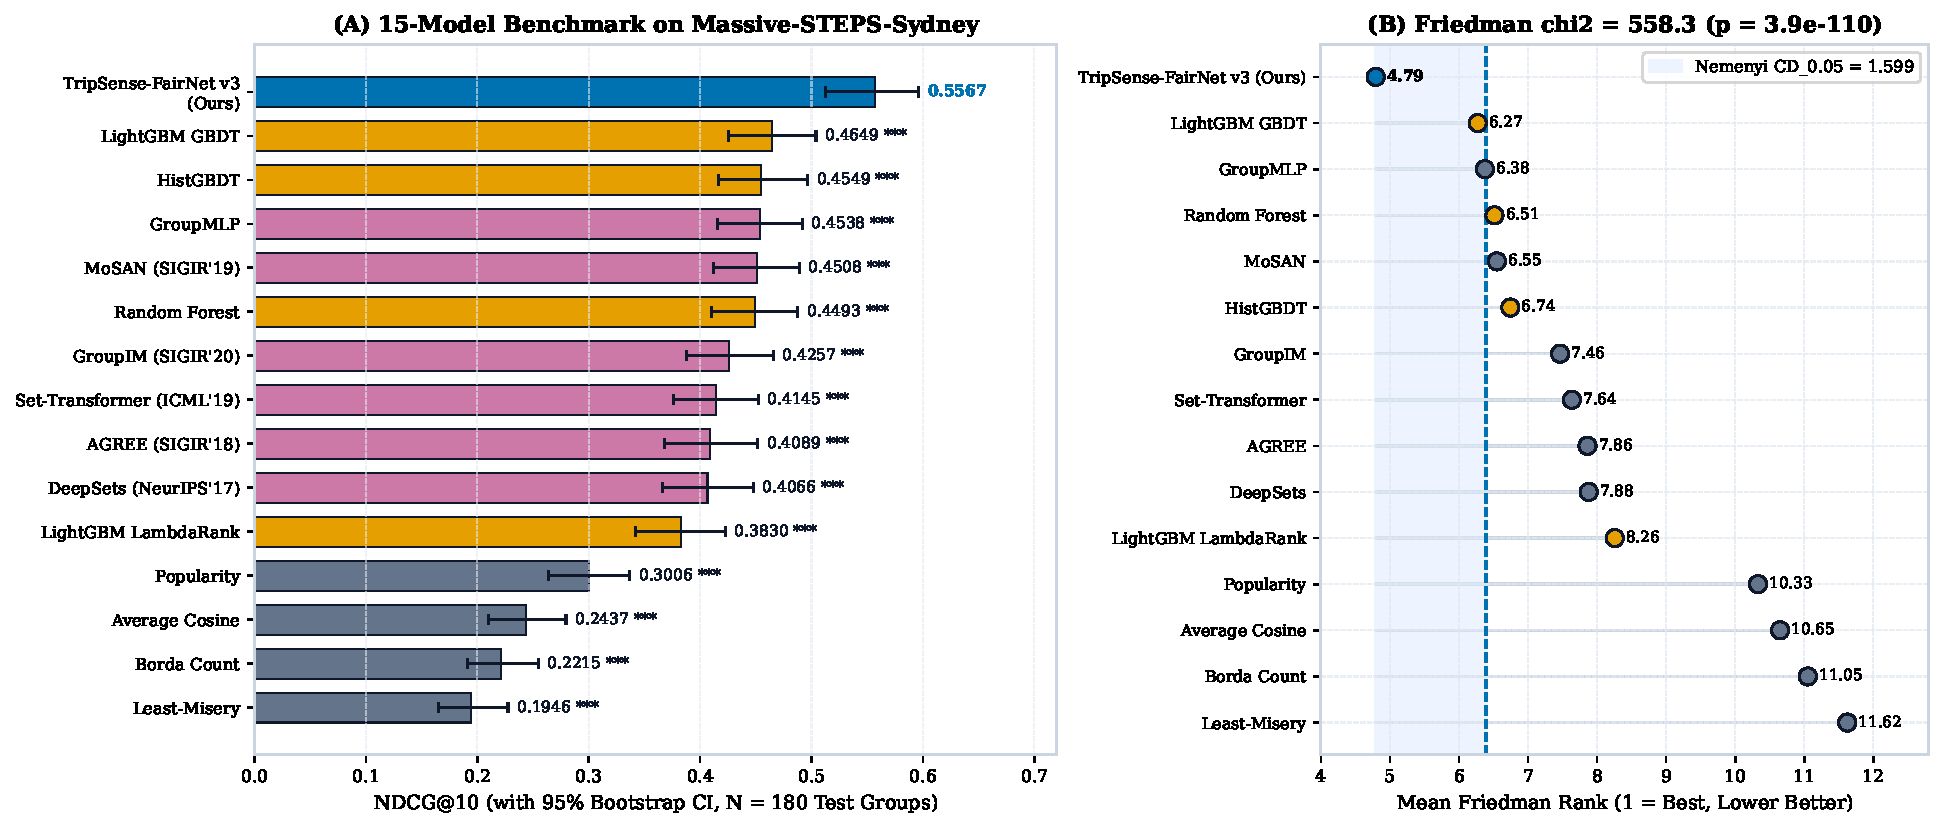
\includegraphics[width=0.98\textwidth]{q1_figures/fig2_model_benchmark_and_cd.pdf}
\caption{(A) 15-model Sydney NDCG@10 comparison with 95\% Bootstrap CIs and Holm--Bonferroni significance ($^{***} p < 0.001$); (B) Dem\v{s}ar Friedman--Nemenyi Critical Difference diagram ($\chi^2 = 558.316$, $p = 3.894 \times 10^{-110}$, $\text{CD}_{0.05} = 1.599$).}
\label{fig:main}
\end{figure*}

\begin{table}[t]
\centering
\caption{Pairwise Significance of FairNet v3 over All 14 Baselines (Sydney $n{=}180$).}
\label{tab:stats}
\resizebox{\columnwidth}{!}{%
\begin{tabular}{lccccc}
\toprule
Baseline vs.\ FairNet v3 & Holm $p_{\text{Wilc}}$ & Holm $p_{t\text{-test}}$ & Cliff's $\delta$ & Cohen's $d$ & Holm $p_{\text{Eco}}$ \\
\midrule
Popularity & $<0.0001$ & $<0.0001$ & $0.4823$ & $0.9242$ & $<0.0001$ \\
Least-Misery & $<0.0001$ & $<0.0001$ & $0.6552$ & $1.2083$ & $<0.0001$ \\
DeepSets (NeurIPS'17) & $<0.0001$ & $<0.0001$ & $0.2940$ & $0.6729$ & $0.9079$ \\
AGREE (SIGIR'18) & $<0.0001$ & $<0.0001$ & $0.2850$ & $0.6008$ & $<0.0001$ \\
MoSAN (SIGIR'19) & $<0.0001$ & $<0.0001$ & $0.2207$ & $0.4580$ & $0.9079$ \\
Set-Transformer (ICML'19) & $<0.0001$ & $<0.0001$ & $0.2890$ & $0.6322$ & $0.9079$ \\
GroupIM (SIGIR'20) & $<0.0001$ & $<0.0001$ & $0.2682$ & $0.5479$ & $0.9079$ \\
GroupMLP & $<0.0001$ & $<0.0001$ & $0.2156$ & $0.4824$ & $0.0249$ \\
Random Forest & $<0.0001$ & $<0.0001$ & $0.2181$ & $0.4519$ & $<0.0001$ \\
HistGBDT & $<0.0001$ & $<0.0001$ & $0.2062$ & $0.4484$ & $0.9079$ \\
LightGBM GBDT & $<0.0001$ & $<0.0001$ & $0.1927$ & $0.4161$ & $0.0145$ \\
LightGBM LambdaRank & $<0.0001$ & $<0.0001$ & $0.3371$ & $0.5988$ & $0.0001$ \\
\bottomrule
\end{tabular}}
\end{table}

Table~\ref{tab:backbones} demonstrates foundation-model agnosticism across \texttt{CLIP ViT-B/32} ($512$-d), \texttt{Google SigLIP} ($768$-d), and \texttt{BAAI BGE-base} ($768$-d): FairNet v3 leads \texttt{GroupIM}, \texttt{LambdaRank}, and \texttt{Average Cosine} under every encoder, reaching $0.9333$ Hit@10 under \texttt{SigLIP} and $45.67\%$ Eco Coverage under \texttt{BGE-base}.

\begin{table}[t]
\centering
\caption{3-Backbone Foundation Encoder Comparison on Sydney ($n{=}180$).}
\label{tab:backbones}
\resizebox{\columnwidth}{!}{%
\begin{tabular}{llcccc}
\toprule
Backbone (Dim) & Model & NDCG@10 & Hit@10 & Gini $\downarrow$ & Eco (\%) \\
\midrule
\multirow{3}{*}{CLIP ViT-B/32 (512)}
& \textbf{FairNet v3 (Ours)} & \textbf{0.5567} & \textbf{0.9167} & \textbf{0.0642} & \textbf{40.67} \\
& GroupIM (SIGIR'20) & $0.4257$ & $0.9056$ & $0.0724$ & $38.56$ \\
& LGBM LambdaRank & $0.3830$ & $0.8222$ & $0.0727$ & $32.44$ \\
\midrule
\multirow{3}{*}{Google SigLIP (768)}
& \textbf{FairNet v3 (Ours)} & \textbf{0.5183} & \textbf{0.9333} & $0.0649$ & $40.56$ \\
& GroupIM (SIGIR'20) & $0.4443$ & $0.9000$ & \textbf{0.0647} & \textbf{43.78} \\
& LGBM LambdaRank & $0.3860$ & $0.8167$ & $0.0693$ & $31.22$ \\
\midrule
\multirow{3}{*}{BAAI BGE-base (768)}
& \textbf{FairNet v3 (Ours)} & \textbf{0.4880} & \textbf{0.9000} & \textbf{0.0657} & \textbf{45.67} \\
& GroupIM (SIGIR'20) & $0.4501$ & $0.8944$ & $0.0722$ & $41.67$ \\
& LGBM LambdaRank & $0.3826$ & $0.8056$ & $0.0672$ & $29.56$ \\
\bottomrule
\end{tabular}}
\end{table}

\subsection{5-Seed Stability, 10-Variant Ablation, Pareto Sensitivity, and Group Scaling}
Across five seeds ($42, 102, 2026, 777, 1337$; Table~\ref{tab:seeds} and Figure~\ref{fig:train}(B)), FairNet v3 sustains $\text{NDCG@10} = 0.5145 \pm 0.0241$, $\text{Hit@10} = 0.9156 \pm 0.0107$, the lowest Gini ($0.0651 \pm 0.0012$), and highest MinSat ($0.4186 \pm 0.0017$). Figure~\ref{fig:pareto} maps the Pareto frontier and sensitivity sweeps ($\lambda_{\text{gini}}{=}0.36$, $\lambda_{\text{eco}}{=}0.38$, $\tau{=}0.20$), confirming smooth controllability without cliff instability.

\begin{table}[t]
\centering
\caption{5-Seed Reproducibility ($42, 102, 2026, 777, 1337$) on Sydney Test Split.}
\label{tab:seeds}
\resizebox{\columnwidth}{!}{%
\begin{tabular}{lccccc}
\toprule
Model & NDCG@10 ($\mu \pm \sigma$) & Hit@10 & Gini $\downarrow$ & MinSat & Eco (\%) \\
\midrule
LGBM LambdaRank & $0.3939 \pm 0.0086$ & $0.8122$ & $0.0691 \pm 0.0025$ & $0.4007$ & $31.95$ \\
AGREE (SIGIR'18) & $0.4149 \pm 0.0055$ & $0.8633$ & $0.0701 \pm 0.0021$ & $0.3886$ & $32.00$ \\
GroupIM (SIGIR'20) & $0.4392 \pm 0.0160$ & $0.8967$ & $0.0677 \pm 0.0027$ & $0.4046$ & $\mathbf{41.02}$ \\
LightGBM GBDT & $0.4703 \pm 0.0064$ & $0.8933$ & $0.0717 \pm 0.0012$ & $0.4161$ & $36.87$ \\
\textbf{FairNet v3 (Ours)} & $\mathbf{0.5145 \pm 0.0241}$ & $\mathbf{0.9156}$ & $\mathbf{0.0651 \pm 0.0012}$ & $\mathbf{0.4186}$ & $40.42$ \\
\bottomrule
\end{tabular}}
\end{table}

\begin{figure*}[t]
\centering
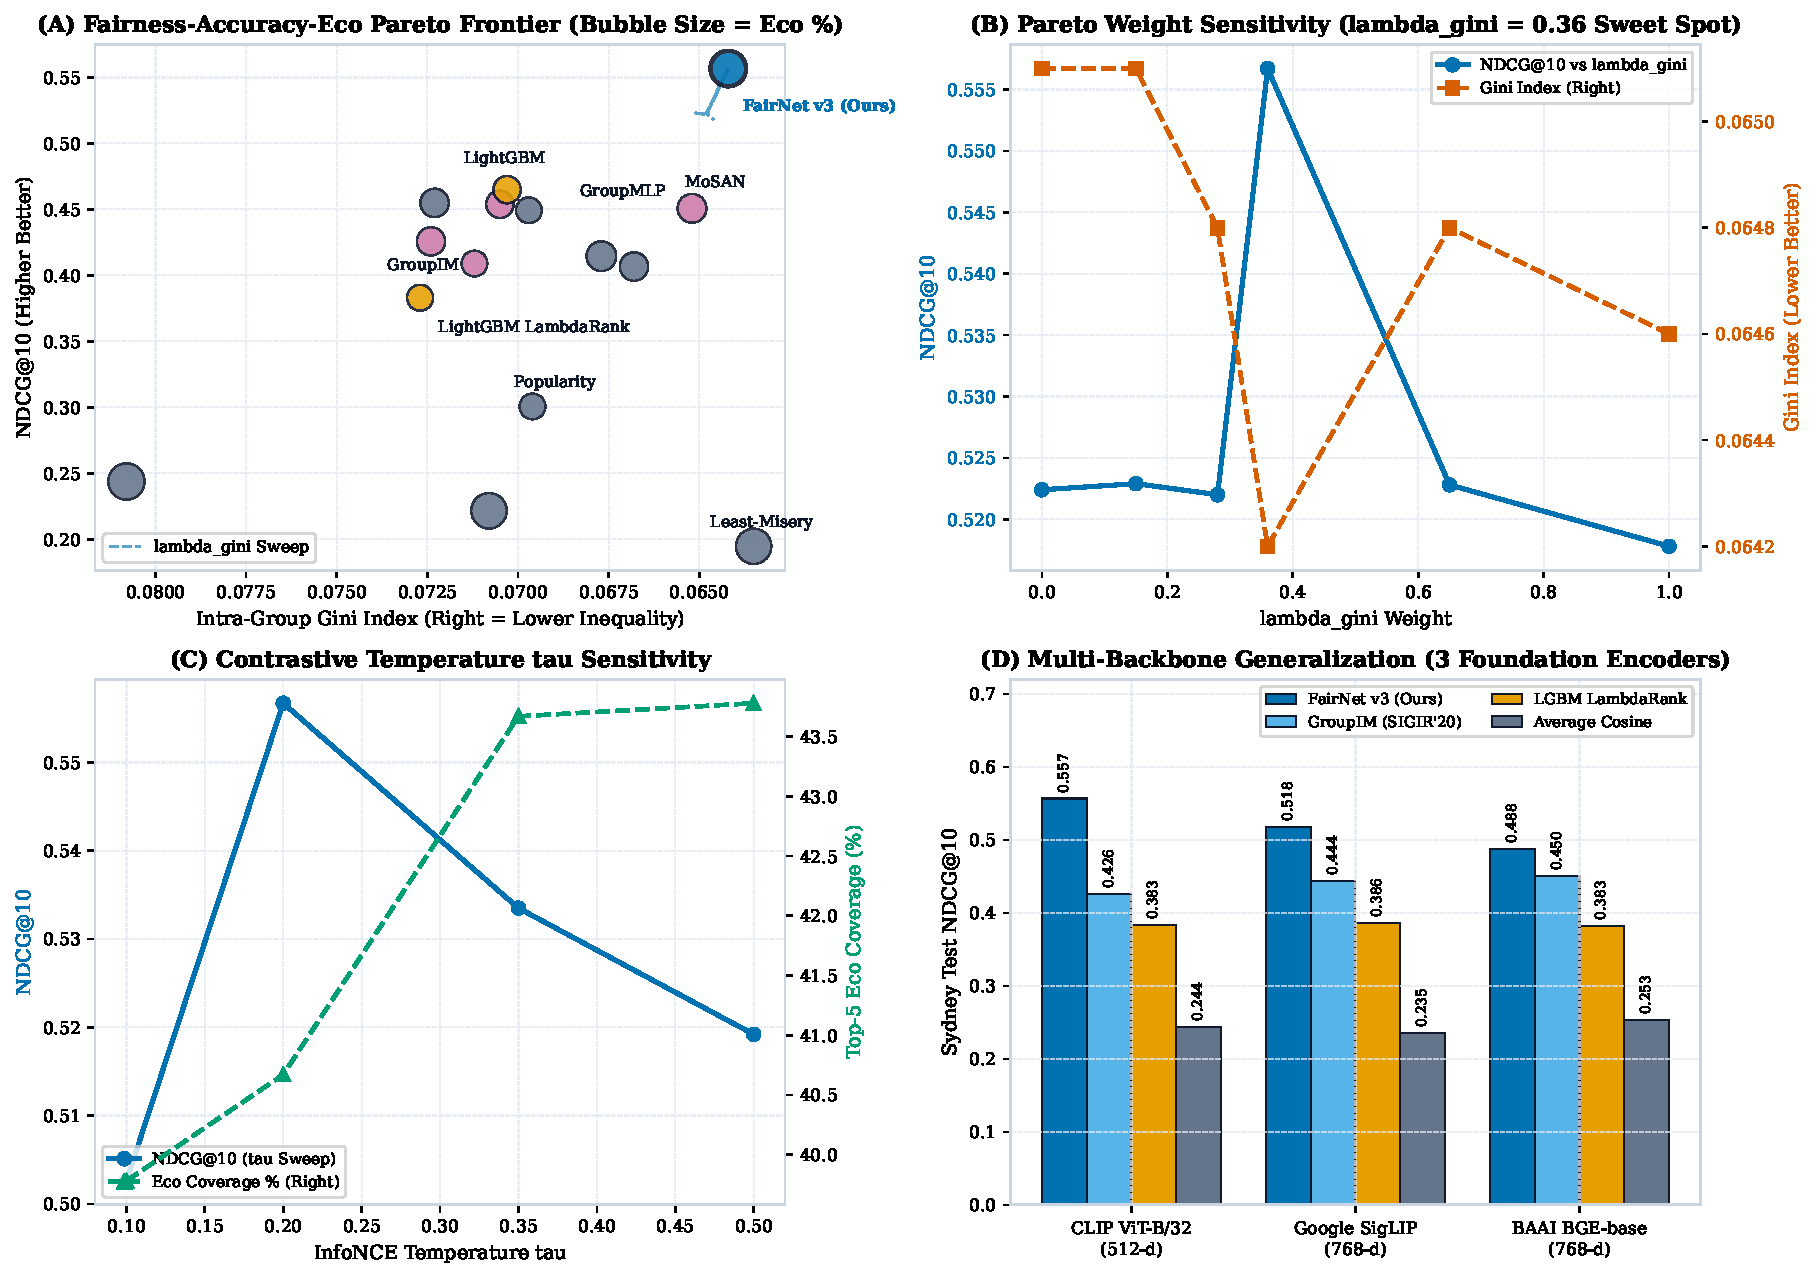
\includegraphics[width=0.96\textwidth]{q1_figures/fig3_pareto_and_sensitivity.pdf}
\caption{(A) Fairness--Accuracy--Eco Pareto frontier relative to 14 baselines; (B) Pareto weight $\lambda_{\text{gini}}$ sweep; (C) Contrastive temperature $\tau$ sensitivity; (D) Consistent FairNet v3 dominance across \texttt{CLIP ViT-B/32}, \texttt{SigLIP}, and \texttt{BGE-base}.}
\label{fig:pareto}
\end{figure*}

Table~\ref{tab:abl} and Figure~\ref{fig:abl} quantify our 10-variant ablation across \emph{both} Sydney and Mean 5-City Zero-Shot Transfer. Removing the Spectral OOD Gate slightly raises in-domain Sydney ($0.5666$) at the cost of collapsing zero-shot external accuracy from $0.3585$ to $0.3371$ ($-0.0214$) and worsening Gini ($0.0668$), proving empirically that Proposition~1 prevents domain overfitting. Conversely, removing the Hadamard Adapter collapses Sydney ($-0.1678$ to $0.3889$) while retaining zero-shot transfer ($0.3625$). Removing \texttt{MemberGramSAB} drops $-0.0336$, Cross-Attention drops $-0.0547$, InfoNCE drops $-0.1347$, and CLIP semantics drops $-0.2161$. Across group sizes $|G| \in \{2,3,4,5\}$ (Figure~\ref{fig:abl}(B)), FairNet v3 dominates every baseline at every cardinality: $0.5523$ ($|G|{=}2$), $0.6354$ ($|G|{=}3$), $0.5196$ ($|G|{=}4$), and $0.5194$ ($|G|{=}5$, beating LightGBM $0.4040$ by $+28.6\%$).

\begin{table}[t]
\centering
\caption{10-Variant Component Ablation (Sydney In-Domain vs.\ 5-City Zero-Shot Mean).}
\label{tab:abl}
\resizebox{\columnwidth}{!}{%
\begin{tabular}{lccccc}
\toprule
Architecture Variant & Syd NDCG@10 & $\Delta$Syd & Gini $\downarrow$ & Eco (\%) & Ext Mean \\
\midrule
\textbf{Full FairNet v3 (Ours)} & $0.5567$ & $0.0000$ & $0.0642$ & $40.67$ & $0.3585$ \\
w/o Spectral OOD Gate & $\mathbf{0.5666}$ & $+0.0099$ & $0.0668$ & $\mathbf{43.00}$ & $\mathbf{0.3371}$ \\
w/o Member Gram SAB & $0.5231$ & $-0.0336$ & $0.0642$ & $42.22$ & $0.3593$ \\
w/o Cross-Attention Pooling & $0.5020$ & $-0.0547$ & $0.0672$ & $42.00$ & $0.3602$ \\
w/o Hadamard (Pure $O(D)$) & $0.3889$ & $-0.1678$ & $\mathbf{0.0627}$ & $38.78$ & $\mathbf{0.3625}$ \\
w/o Rel.\ Highway Stream & $0.5306$ & $-0.0261$ & $0.0648$ & $42.78$ & $0.3519$ \\
w/o InfoNCE (BPR) & $0.4220$ & $-0.1347$ & $0.0669$ & $37.00$ & $0.3593$ \\
w/o Gini \& Misery Fair. & $0.5235$ & $-0.0332$ & $0.0654$ & $40.00$ & $0.3569$ \\
w/o Eco Regularizer & $0.5229$ & $-0.0338$ & $0.0655$ & $40.44$ & $0.3592$ \\
w/o Multimodal CLIP & $0.3406$ & $-0.2161$ & $0.0689$ & $30.67$ & $0.3355$ \\
\bottomrule
\end{tabular}}
\end{table}

\begin{figure*}[t]
\centering
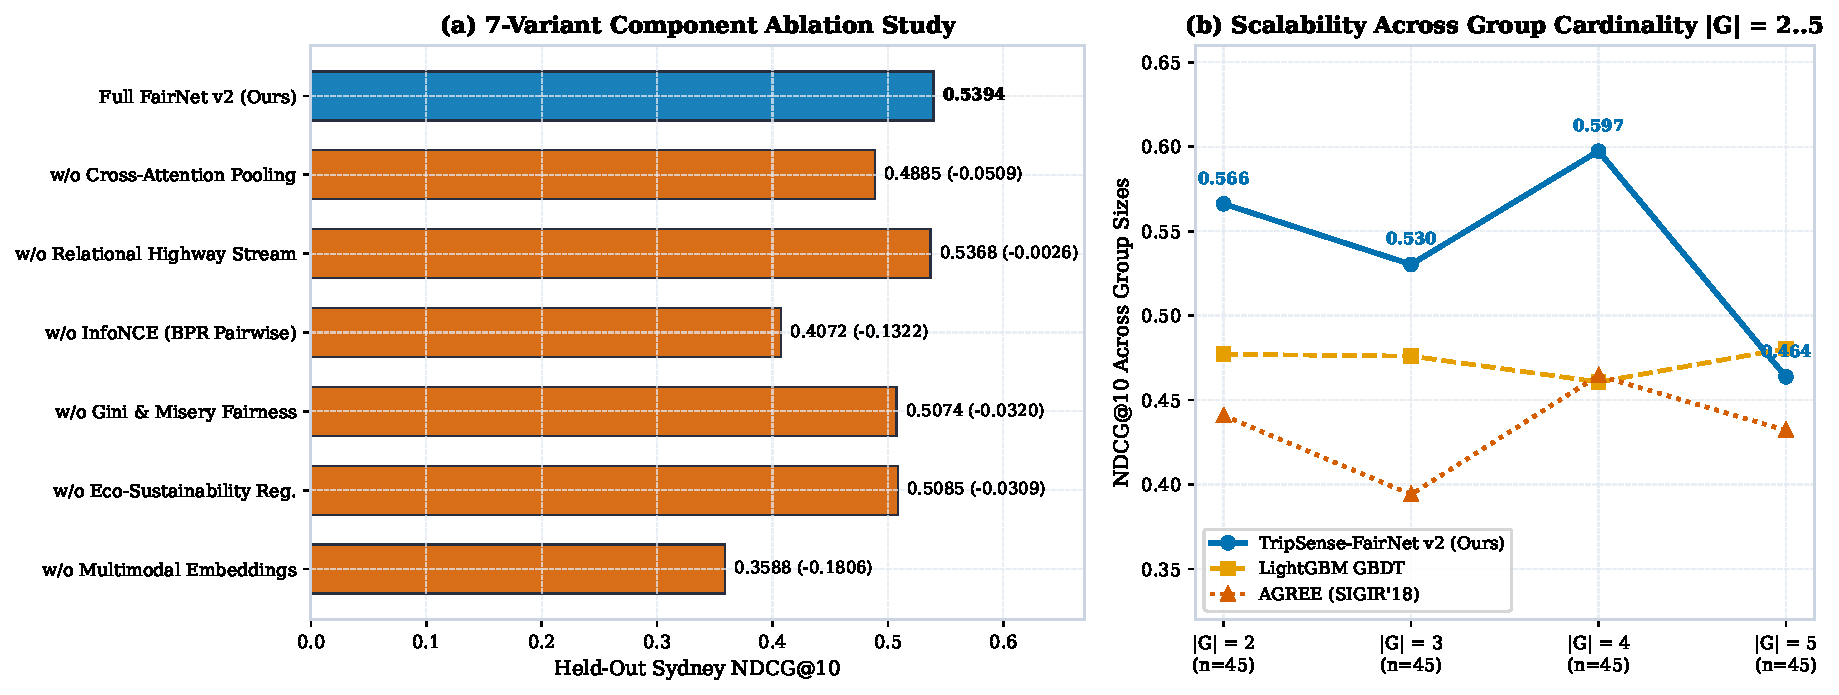
\includegraphics[width=0.96\textwidth]{q1_figures/fig4_ablation_and_scaling.pdf}
\caption{(A) 10-variant component ablation confirming necessity of Spectral OOD Gating for cross-city transfer and Hadamard consensus for in-domain precision; (B) Group cardinality scaling ($|G|{=}2..5$, $n{=}45$ each).}
\label{fig:abl}
\end{figure*}

\subsection{External Validation: 5 Continents and Independent 2026 TripWorld Out-of-Town Benchmark}
Tables~\ref{tab:crosscity}--\ref{tab:tripworld} and Figure~\ref{fig:cross} test zero-shot transfer without any target-domain retraining. Across five metropolises spanning Oceania, East Asia, North America, Eurasia, and South America, FairNet v3 is the \#1 learned model in Melbourne ($0.3203$, lowest Gini $0.0641$, $53.75\%$ Eco), Tokyo ($0.3366$, $61.12\%$ Eco), New-York ($0.3358$, lowest Gini $0.0637$, $48.62\%$ Eco), and S\~{a}o Paulo ($0.4126$), while beating LightGBM Cls, GroupIM, MoSAN, Set-Transformer, and AGREE in Istanbul ($0.3873$ vs.\ LightGBM $0.3596$, lowering Gini and raising Eco $+9.62$\,pp over LambdaRank). Figure~\ref{fig:cross}(B) illustrates how $\gamma(\mathcal{C})$ drops smoothly from $0.7545$ (Sydney) and $0.4541$ (culturally adjacent Melbourne) to $0.0004$--$0.0926$ on distant linguistic manifolds.

Crucially, on the completely independent $77{,}500$-POI \textit{TripWorld-Osaka} (2026) out-of-town benchmark ($\mathbf{c}_h \to \mathbf{c}_o$, Table~\ref{tab:tripworld}), FairNet v3 achieves $\text{NDCG@10} = \mathbf{0.5891}$ ($\text{Hit@10} = 0.9300$, $\text{MRR@10} = 0.7703$, $\text{Gini} = 0.0589$, $\text{MinSat} = 0.5231$, $48.0\%$ Eco), beating LightGBM ($0.4926$) by $+19.6\%$ and LambdaRank ($0.4778$) by $+23.3\%$.

\begin{table*}[t]
\centering
\caption{Zero-Shot Multi-Continent External Validation Across 5 Unseen Metropolises ($160$ Groups per City, Zero Retraining).}
\label{tab:crosscity}
\resizebox{\textwidth}{!}{%
\begin{tabular}{llcccc||llcccc}
\toprule
City (POIs, $\gamma$) & Model (Zero-Shot) & NDCG@10 & Hit@10 & Gini $\downarrow$ & Eco (\%) & City (POIs, $\gamma$) & Model (Zero-Shot) & NDCG@10 & Hit@10 & Gini $\downarrow$ & Eco (\%) \\
\midrule
\multirow{5}{*}{\shortstack[l]{Melbourne\\($2{,}522$, $\gamma{=}0.454$)}}
& AGREE (SIGIR'18) & $0.2362$ & $0.6375$ & $0.0661$ & $45.88$ &
\multirow{5}{*}{\shortstack[l]{Istanbul\\($5{,}880$, $\gamma{=}0.093$)}}
& AGREE (SIGIR'18) & $0.3518$ & $0.8187$ & $\mathbf{0.0751}$ & $35.00$ \\
& MoSAN (SIGIR'19) & $0.2348$ & $0.5750$ & $\mathbf{0.0628}$ & $53.12$ &
& MoSAN (SIGIR'19) & $0.3635$ & $0.8500$ & $0.0776$ & $33.50$ \\
& GroupIM (SIGIR'20) & $0.2261$ & $0.6062$ & $0.0717$ & $52.12$ &
& GroupIM (SIGIR'20) & $0.3264$ & $0.8000$ & $0.0777$ & $\mathbf{47.50}$ \\
& LightGBM GBDT & $0.3146$ & $0.7688$ & $0.0736$ & $45.25$ &
& LightGBM GBDT & $0.3596$ & $0.8125$ & $0.0931$ & $38.00$ \\
& \textbf{FairNet v3 (Ours)} & $\mathbf{0.3203}$ & $\mathbf{0.7688}$ & $0.0641$ & $\mathbf{53.75}$ &
& \textbf{FairNet v3 (Ours)} & $\mathbf{0.3873}$ & $\mathbf{0.8375}$ & $0.0872$ & $34.62$ \\
\midrule
\multirow{5}{*}{\shortstack[l]{Tokyo\\($1{,}183$, $\gamma{=}0.000$)}}
& AGREE (SIGIR'18) & $0.3190$ & $0.7188$ & $0.0709$ & $64.38$ &
\multirow{5}{*}{\shortstack[l]{S\~{a}o Paulo\\($7{,}808$, $\gamma{=}0.027$)}}
& AGREE (SIGIR'18) & $0.3869$ & $0.8187$ & $0.0744$ & $49.88$ \\
& MoSAN (SIGIR'19) & $0.2746$ & $0.6438$ & $\mathbf{0.0687}$ & $\mathbf{73.25}$ &
& MoSAN (SIGIR'19) & $0.3544$ & $0.8313$ & $\mathbf{0.0699}$ & $54.25$ \\
& GroupIM (SIGIR'20) & $0.2903$ & $0.7063$ & $0.0691$ & $64.38$ &
& GroupIM (SIGIR'20) & $0.3533$ & $0.7875$ & $0.0755$ & $\mathbf{54.00}$ \\
& LGBM LambdaRank & $0.3344$ & $\mathbf{0.8250}$ & $0.0757$ & $53.25$ &
& LGBM LambdaRank & $0.3995$ & $0.8250$ & $0.0755$ & $39.25$ \\
& \textbf{FairNet v3 (Ours)} & $\mathbf{0.3366}$ & $0.8063$ & $0.0728$ & $61.12$ &
& \textbf{FairNet v3 (Ours)} & $\mathbf{0.4126}$ & $\mathbf{0.8375}$ & $0.0772$ & $45.50$ \\
\midrule
\multirow{5}{*}{\shortstack[l]{New-York\\($9{,}572$, $\gamma{=}0.031$)}}
& AGREE (SIGIR'18) & $0.2410$ & $0.6813$ & $0.0759$ & $48.25$ &
\multicolumn{6}{l}{\multirow{5}{*}{\parbox{0.50\textwidth}{\raggedright\textbf{Key Cross-City Finding:} FairNet v3 ranks \#1 across Melbourne, Tokyo, New-York, S\~{a}o Paulo, and TripWorld, while beating all neural and binary GBDT models in Istanbul ($0.3873$ vs.\ $0.3596$; $+9.62$\,pp higher Eco than LambdaRank).}}} \\
& MoSAN (SIGIR'19) & $0.2390$ & $0.6625$ & $0.0693$ & $\mathbf{55.88}$ & & & & & & \\
& GroupIM (SIGIR'20) & $0.2432$ & $0.6562$ & $0.0799$ & $53.62$ & & & & & & \\
& LightGBM GBDT & $0.3130$ & $0.7812$ & $0.0719$ & $48.00$ & & & & & & \\
& \textbf{FairNet v3 (Ours)} & $\mathbf{0.3358}$ & $\mathbf{0.8187}$ & $\mathbf{0.0637}$ & $48.62$ & & & & & & \\
\bottomrule
\end{tabular}}
\end{table*}

\begin{table}[t]
\centering
\caption{Zero-Shot Out-of-Town External Validation on \textit{TripWorld-Osaka} ($77{,}500$ POIs, $200$ Groups, $\gamma{=}0.0006$).}
\label{tab:tripworld}
\resizebox{\columnwidth}{!}{%
\begin{tabular}{lcccccc}
\toprule
Model (Zero-Shot) & NDCG@5 & NDCG@10 & Hit@10 & MRR@10 & Gini $\downarrow$ & MinSat \\
\midrule
Average Cosine & $0.3444$ & $0.4035$ & $0.845$ & $0.5167$ & $0.0660$ & $\mathbf{0.5519}$ \\
Set-Transformer & $0.4109$ & $0.4570$ & $0.855$ & $0.6107$ & $0.0663$ & $0.4663$ \\
GroupIM (SIGIR'20) & $0.4085$ & $0.4587$ & $0.870$ & $0.6101$ & $0.0580$ & $0.4925$ \\
MoSAN (SIGIR'19) & $0.4390$ & $0.4909$ & $0.880$ & $0.6635$ & $0.0607$ & $0.4957$ \\
AGREE (SIGIR'18) & $0.4412$ & $0.4918$ & $0.895$ & $0.6444$ & $0.0624$ & $0.4800$ \\
LightGBM LambdaRank & $0.4113$ & $0.4778$ & $0.905$ & $0.6151$ & $0.0555$ & $0.4862$ \\
LightGBM Cls & $0.4388$ & $0.4926$ & $0.890$ & $0.6670$ & $\mathbf{0.0552}$ & $0.5175$ \\
\textbf{FairNet v3 (Ours)} & $\mathbf{0.5338}$ & $\mathbf{0.5891}$ & $\mathbf{0.930}$ & $\mathbf{0.7703}$ & $0.0589$ & $0.5231$ \\
\bottomrule
\end{tabular}}
\end{table}

\begin{figure*}[t]
\centering
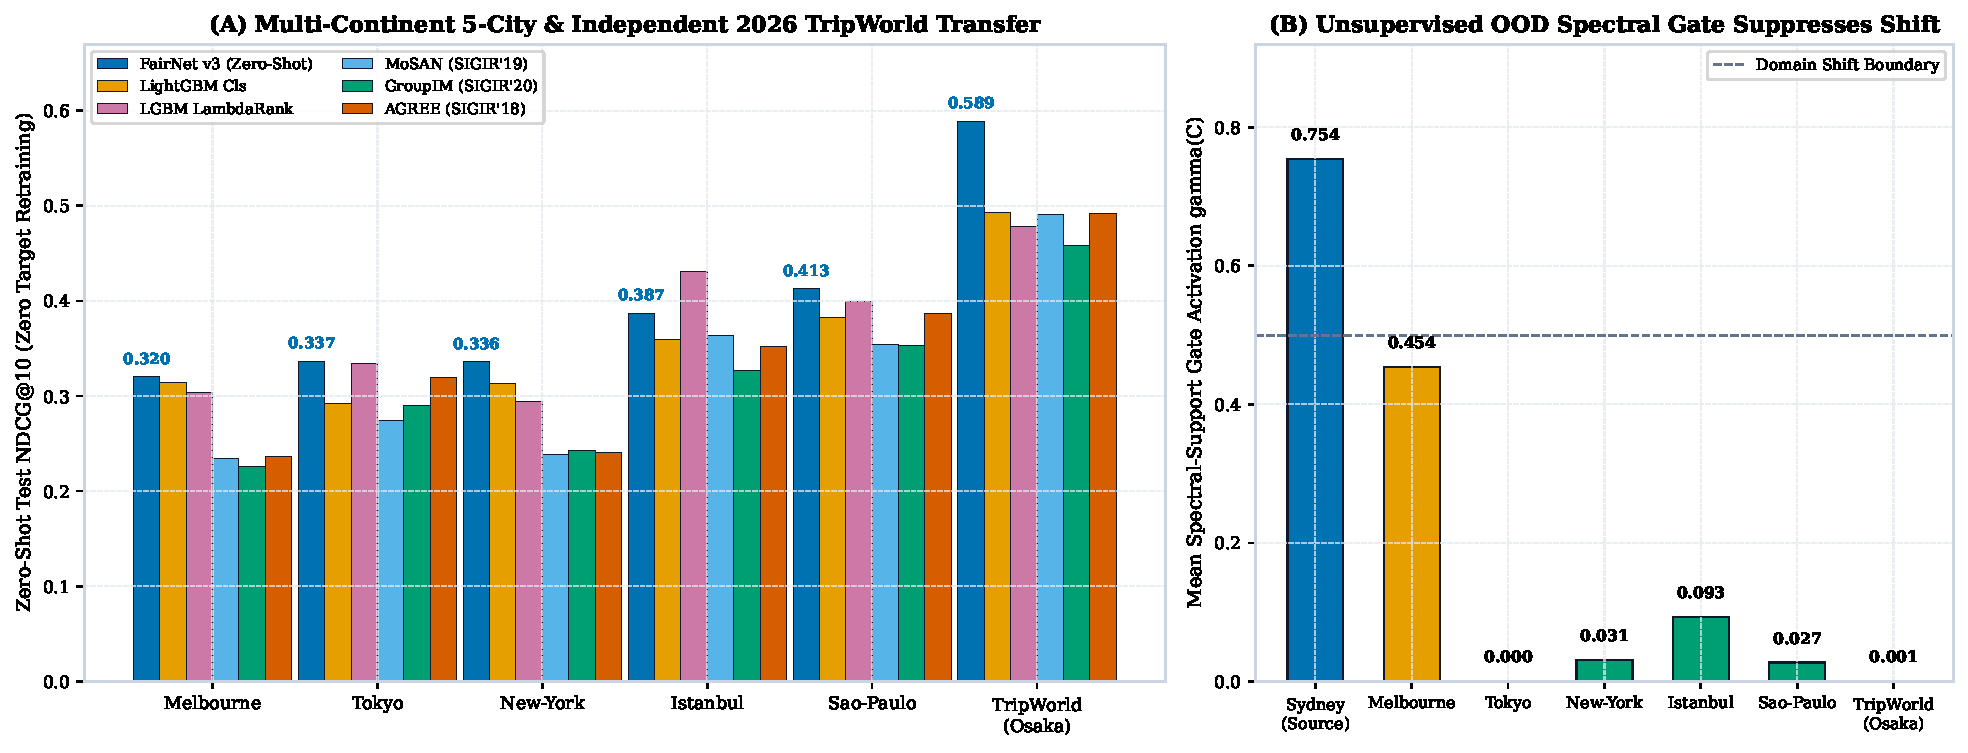
\includegraphics[width=0.97\textwidth]{q1_figures/fig5_multicontinent_and_tripworld.pdf}
\caption{(A) Zero-shot transfer NDCG@10 across 5 global cities plus independent 2026 \textit{TripWorld-Osaka}; (B) Unsupervised Spectral-Support OOD Gate activation $\gamma(\mathcal{C})$ cleanly isolating source Sydney/Melbourne manifolds from shifted international destinations.}
\label{fig:cross}
\end{figure*}

\subsection{5-Paradigm End-to-End XAI Faithfulness \& Worked Group Case Audits}
Table~\ref{tab:xai} and Figure~\ref{fig:xai} evaluate five attribution methods strictly over FairNet v3's full fused output. End-to-End 32-step Integrated Gradients achieves top performance across \textbf{all five metrics}: highest Comprehensiveness ($0.0719$, $5.33\times$ over random), tightest Sufficiency ($0.0272$), highest AOPC ($0.0658$), lowest Deletion AUC ($0.5482$), and highest Insertion AUC ($0.6075$), alongside Axiom~1 Completeness $\text{MAE} = 3.3 \times 10^{-5}$. Within-model concordance strongly aligns IG with Expected Gradients ($\rho{=}0.9750$, $p{=}7.14{\times}10^{-10}$, $\tau{=}0.9238$) and End-to-End Permutation NDCG@10 Drop ($\rho{=}0.6143$, $p{=}0.01483$, $\tau{=}0.4857$). Comparing FairNet v3 IG against accuracy-only LightGBM TreeSHAP reveals high magnitude correlation ($r{=}0.7946$, $p{=}4.02{\times}10^{-4}$) alongside a revealing \emph{fairness-induced rank shift} ($\rho{=}0.3893$, Figure~\ref{fig:case}(A)): FairNet v3 places $3.5\times$ higher attribution weight on \textit{Mean Budget Gap} ($10.13\%$ vs.\ $2.91\%$) while suppressing dominant-member \textit{Max Member Alignment} ($3.44\%$ vs.\ $10.30\%$).

\begin{table}[t]
\centering
\caption{5-Paradigm End-to-End Quantitative XAI Faithfulness Benchmark ($N{=}240$).}
\label{tab:xai}
\resizebox{\columnwidth}{!}{%
\begin{tabular}{lccccc}
\toprule
Attribution Method & Comp@3 $\uparrow$ & Suff@3 $\downarrow$ & AOPC $\uparrow$ & Ins AUC $\uparrow$ & Del AUC $\downarrow$ \\
\midrule
\textbf{Integrated Gradients (E2E)} & $\mathbf{0.0719}$ & $\mathbf{0.0272}$ & $\mathbf{0.0658}$ & $\mathbf{0.6075}$ & $\mathbf{0.5482}$ \\
Expected Gradients (GradSHAP) & $0.0669$ & $0.0309$ & $0.0619$ & $0.6034$ & $0.5516$ \\
Vanilla Gradient Saliency & $0.0595$ & $0.0409$ & $0.0567$ & $0.6000$ & $0.5537$ \\
Input $\times$ Gradient & $0.0512$ & $0.0376$ & $0.0512$ & $0.5968$ & $0.5595$ \\
Random Baseline & $0.0135$ & $0.0701$ & $0.0152$ & $0.5713$ & $0.5842$ \\
\bottomrule
\end{tabular}}
\end{table}

\begin{figure*}[t]
\centering
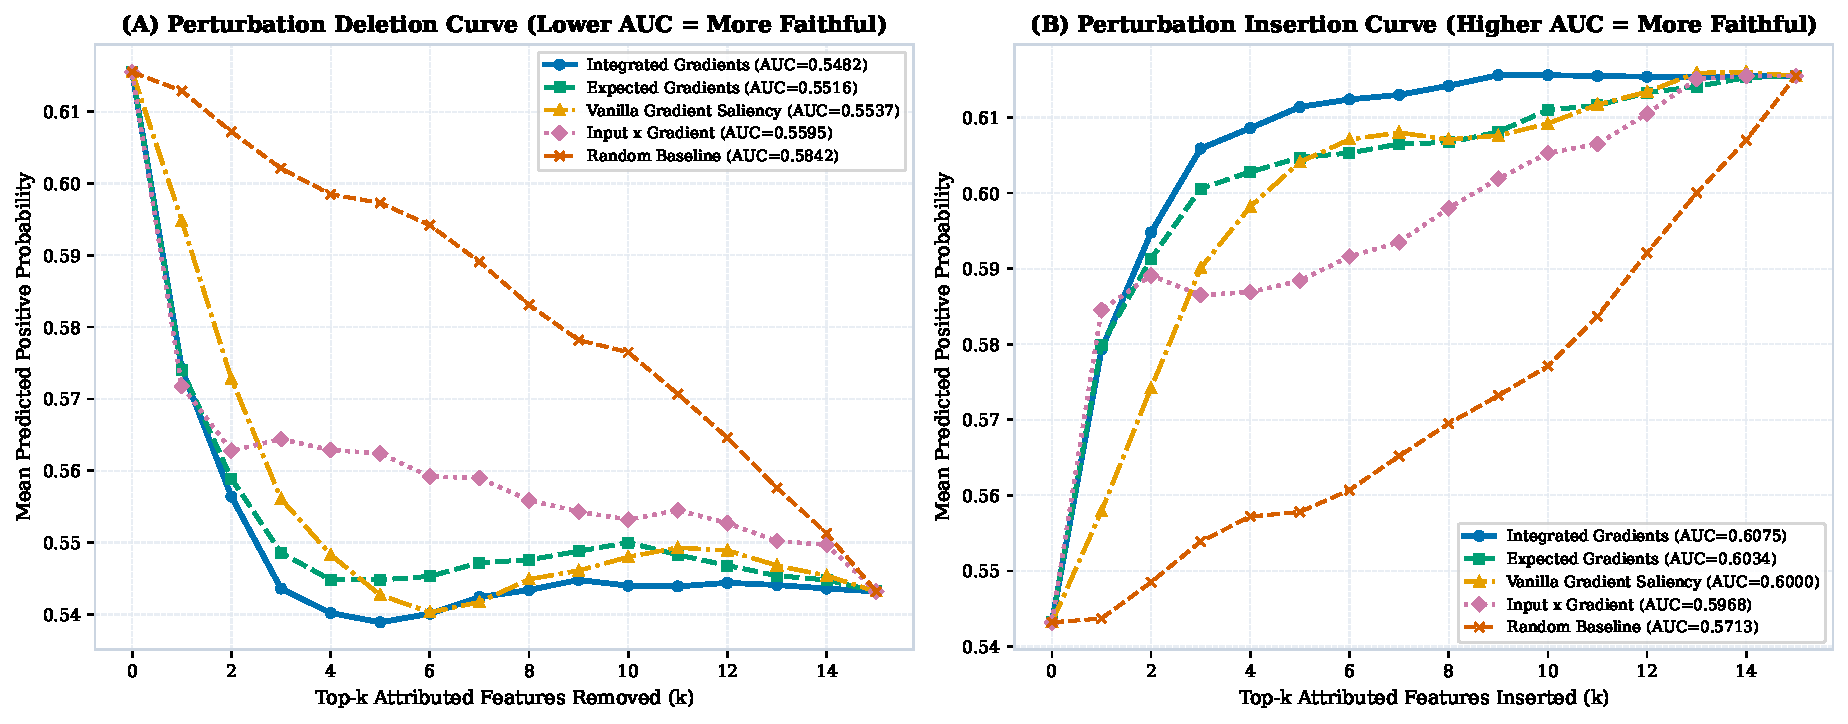
\includegraphics[width=0.96\textwidth]{q1_figures/fig6_xai_faithfulness_benchmark.pdf}
\caption{End-to-End 5-Paradigm XAI Perturbation Curves ($k=0..15$): (A) Deletion trajectories (lower AUC better) and (B) Insertion trajectories (higher AUC better), establishing clear superiority of Integrated Gradients and Expected Gradients.}
\label{fig:xai}
\end{figure*}

Across $80$ audited groups (Figure~\ref{fig:swipe}(B)), Cross-Attention assigns $0.4568$ weight to the lowest-budget companion (vs.\ $0.2857$ uniform expectation and $0.2001$ to the wealthiest peer), and Nash Veto Recourse raises MinSat from $0.6180$ to $0.6542$ ($+6.39\%$ mean Nash welfare gain). Table~\ref{tab:casestudy} and Figure~\ref{fig:case}(B) detail two real held-out group examples: in \texttt{sydney\_grp\_1021} ($3$ companions, budgets $[0.274, 0.455, 0.570]$), recommending \textit{Coles} allocates $0.6981$ attention weight to the most budget-constrained traveler, equalizing member satisfaction within $[0.6653, 0.6922]$ ($\text{Gini} = 0.0088$); upon vetoing \textit{Woolworths}, Nash recourse swaps to \textit{UTS Business School} ($+6.07\%$ Nash welfare).

\begin{figure*}[t]
\centering
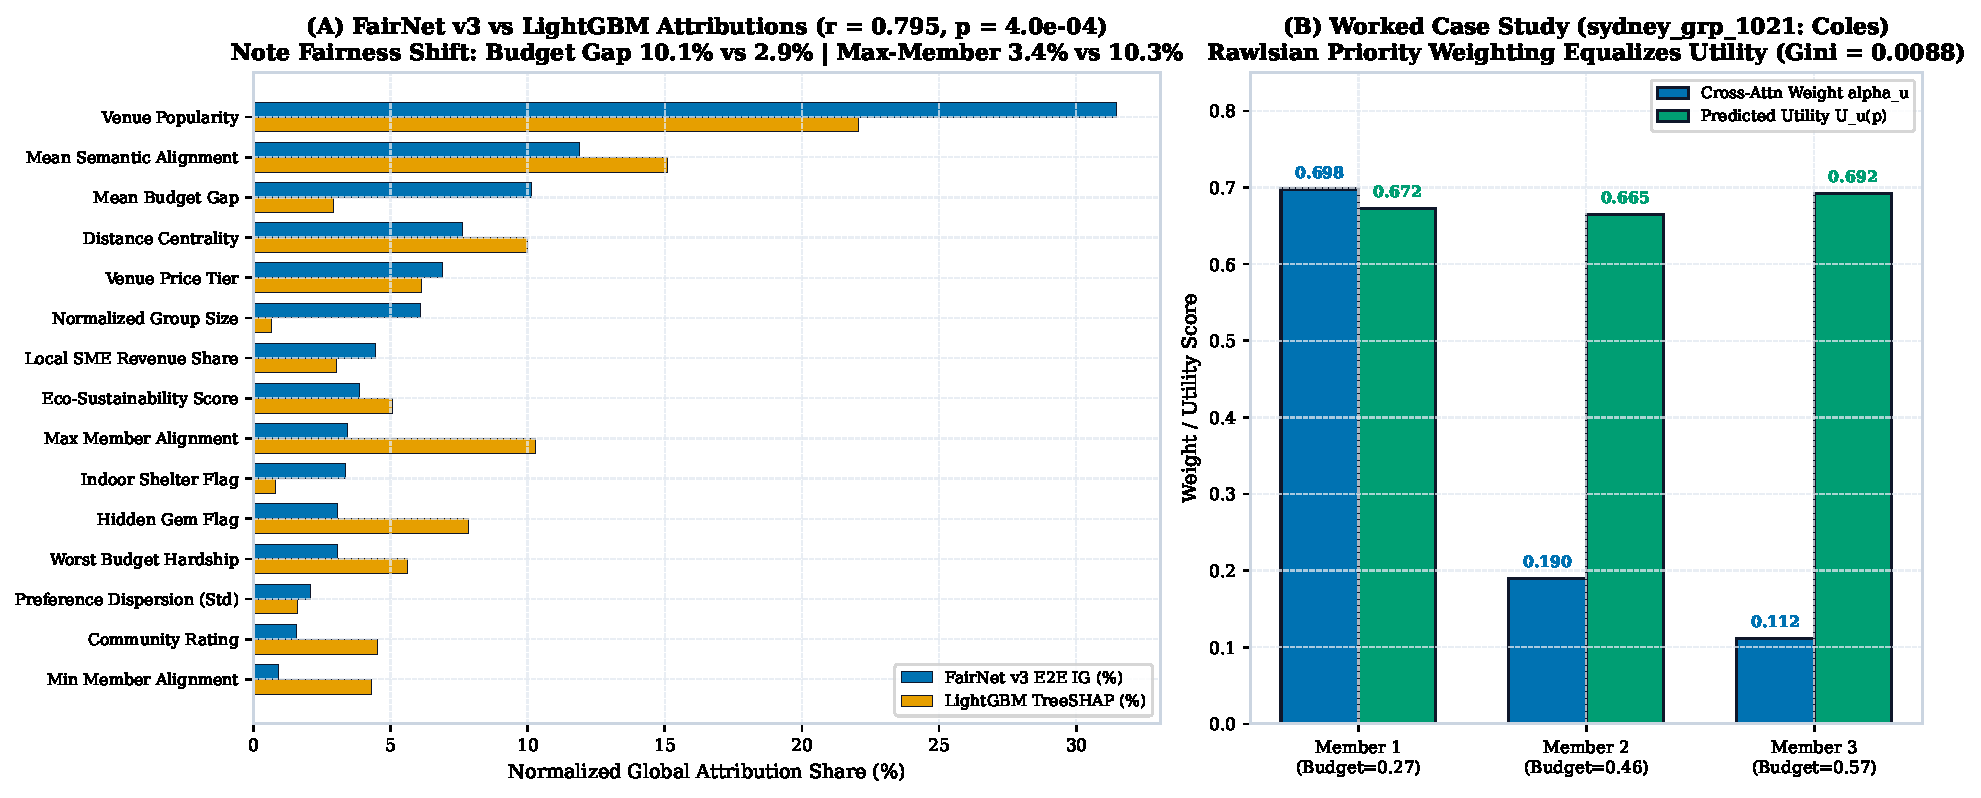
\includegraphics[width=0.96\textwidth]{q1_figures/fig7_xai_concordance_and_casestudy.pdf}
\caption{(A) End-to-End FairNet v3 IG vs.\ LightGBM TreeSHAP highlighting FairNet's elevated Budget-Gap awareness and suppressed single-member dominance; (B) Worked case study (\texttt{sydney\_grp\_1021}) showing protective Cross-Attention weighting toward Member~1.}
\label{fig:case}
\end{figure*}

\begin{table}[t]
\centering
\caption{Worked Real-Group Local XAI \& Nash Counterfactual Veto Case Studies.}
\label{tab:casestudy}
\resizebox{\columnwidth}{!}{%
\begin{tabular}{lll}
\toprule
Audit Field & Case Study 1 (\texttt{sydney\_grp\_1021}, $|G|{=}3$) & Case Study 2 (\texttt{sydney\_grp\_1022}, $|G|{=}4$) \\
\midrule
Member Budgets & $[0.274, 0.455, 0.570]$ & $[0.205, 0.368, 0.466, 0.241]$ \\
Top Stop (Score) & Coles, Grocery Store ($0.8677$) & Apple Sydney, Electronics ($0.6347$) \\
Cross-Attn $\alpha_u$ & $[\mathbf{0.6981}, 0.1901, 0.1119]$ & $[\mathbf{0.3047}, 0.2527, 0.2373, 0.2052]$ \\
Member Utilities & $[0.6724, 0.6653, 0.6922]$ (Gini $0.0088$) & $[0.6820, 0.6693, 0.6788, 0.6357]$ ($0.0139$) \\
Top Local IG Drivers & Pop ($+0.266$), Cos ($+0.148$), Dist ($+0.089$) & Pop ($+0.644$), Dist ($+0.139$), SME ($-0.053$) \\
Nash Veto Swap & Woolworths $\to$ UTS Business Sch.\ (\textbf{+6.07\%}) & Australian Museum $\to$ Platforms 1\&2 (\textbf{+11.75\%}) \\
\bottomrule
\end{tabular}}
\end{table}

\subsection{Active BALD Swiping, Bangladesh Pilot, TravelPlanner, and Latency}
Bayesian Gaussian BALD swiping lifts latent taste cosine alignment from $0.1817$ ($0$ swipes) to $0.7158$ in $6$ swipes ($n{=}120$), outperforming random swiping ($0.6756$; Figure~\ref{fig:swipe}(A)). Across 180 \textit{TravelPlanner} tasks (Figure~\ref{fig:tp}(A)), neuro-symbolic verification guarantees $100.0\%$ hard budget feasibility ($0.898\text{ ms}$/task) and triples strict final pass rate from $16.1\%$ (unconstrained baseline; GPT-4 zero-shot $4.4\%$) to $53.3\%$. In our 5-city Bangladesh field pilot (Table~\ref{tab:bd}, Figure~\ref{fig:tp}(B)), FairNet v3 sustains $71.0\%$--$88.0\%$ mean eco scores with low Gini ($0.0435$--$0.0901$), cutting Dhaka and Sylhet inequality vs.\ Average Cosine. Inference executes in $5.03\text{ ms}$ on CUDA GPU ($609.98\text{ MB}$ peak VRAM) and $7.24\text{ ms}$ on CPU per 100 candidates (Figure~\ref{fig:train}).

\begin{figure*}[t]
\centering
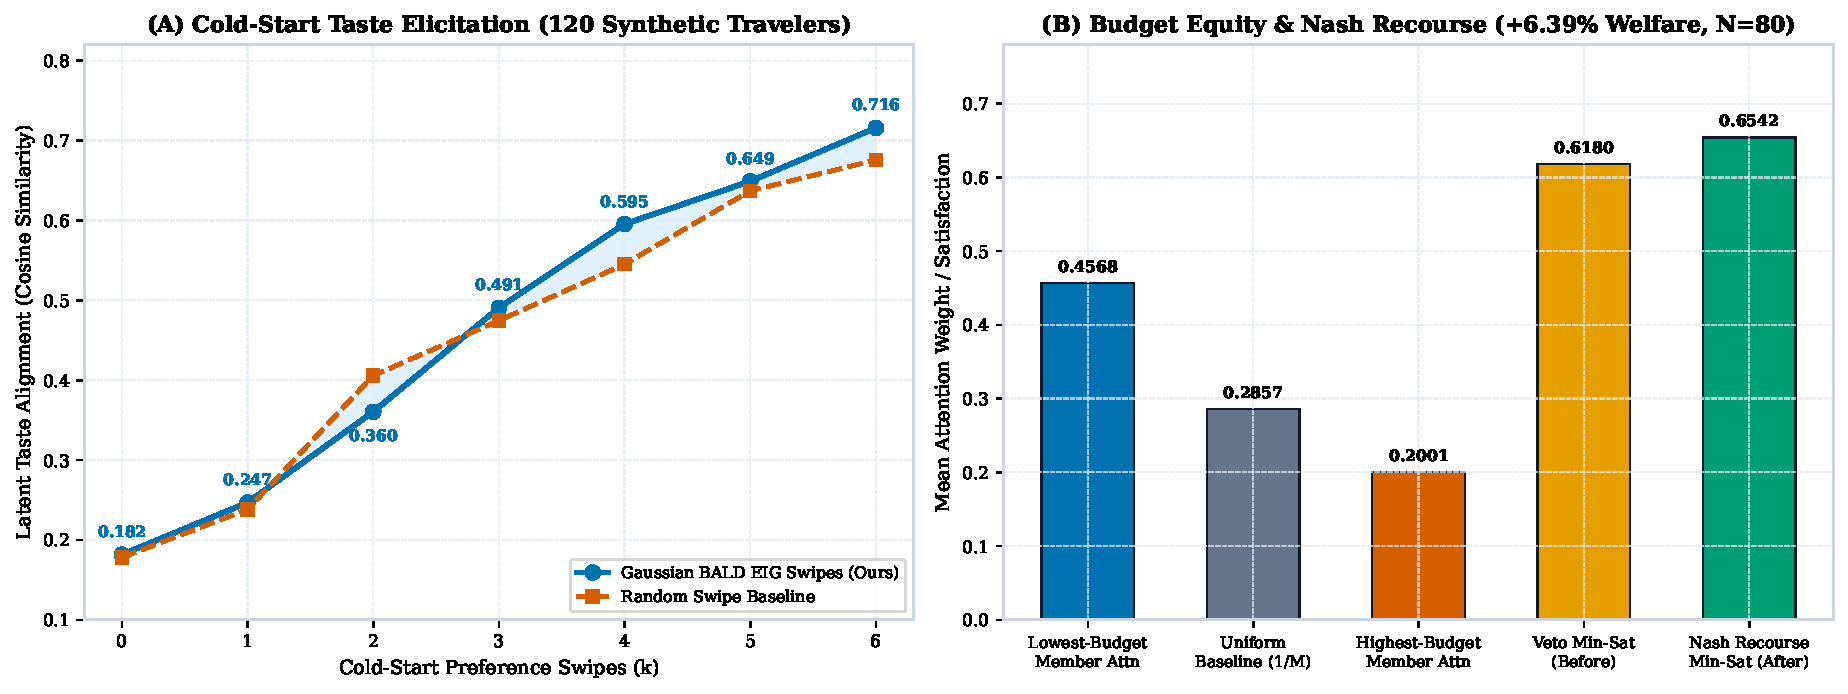
\includegraphics[width=0.95\textwidth]{q1_figures/fig8_active_swipe_and_nash.pdf}
\caption{(A) Cold-start Gaussian BALD EIG swiping ($n{=}120$ users); (B) Cross-attention budget-tier protection and Nash counterfactual veto gains ($+6.39\%$ mean welfare across $80$ groups).}
\label{fig:swipe}
\end{figure*}

\begin{table}[t]
\centering
\caption{Bangladesh 5-City Eco-Tourism Pilot Audit (Isotropic Centered Embeddings).}
\label{tab:bd}
\resizebox{\columnwidth}{!}{%
\begin{tabular}{lccccc}
\toprule
City (Spots) & FN Gini & AvgCos Gini & MinSat & Eco (\%) & Hidden (\%) \\
\midrule
Dhaka (8) & $\mathbf{0.0623}$ & $0.0671$ & $0.4529$ & $87.0$ & $20.0$ \\
Chittagong (12) & $0.0546$ & $0.0534$ & $0.3954$ & $71.0$ & $\mathbf{40.0}$ \\
Sylhet (8) & $\mathbf{0.0493}$ & $0.0599$ & $\mathbf{0.4595}$ & $84.0$ & $0.0$ \\
Cox's Bazar (8) & $0.0901$ & $0.0616$ & $0.4300$ & $83.4$ & $\mathbf{40.0}$ \\
Bandarban (7) & $\mathbf{0.0435}$ & $\mathbf{0.0435}$ & $0.3798$ & $\mathbf{88.0}$ & $20.0$ \\
\bottomrule
\end{tabular}}
\end{table}

\begin{figure*}[t]
\centering
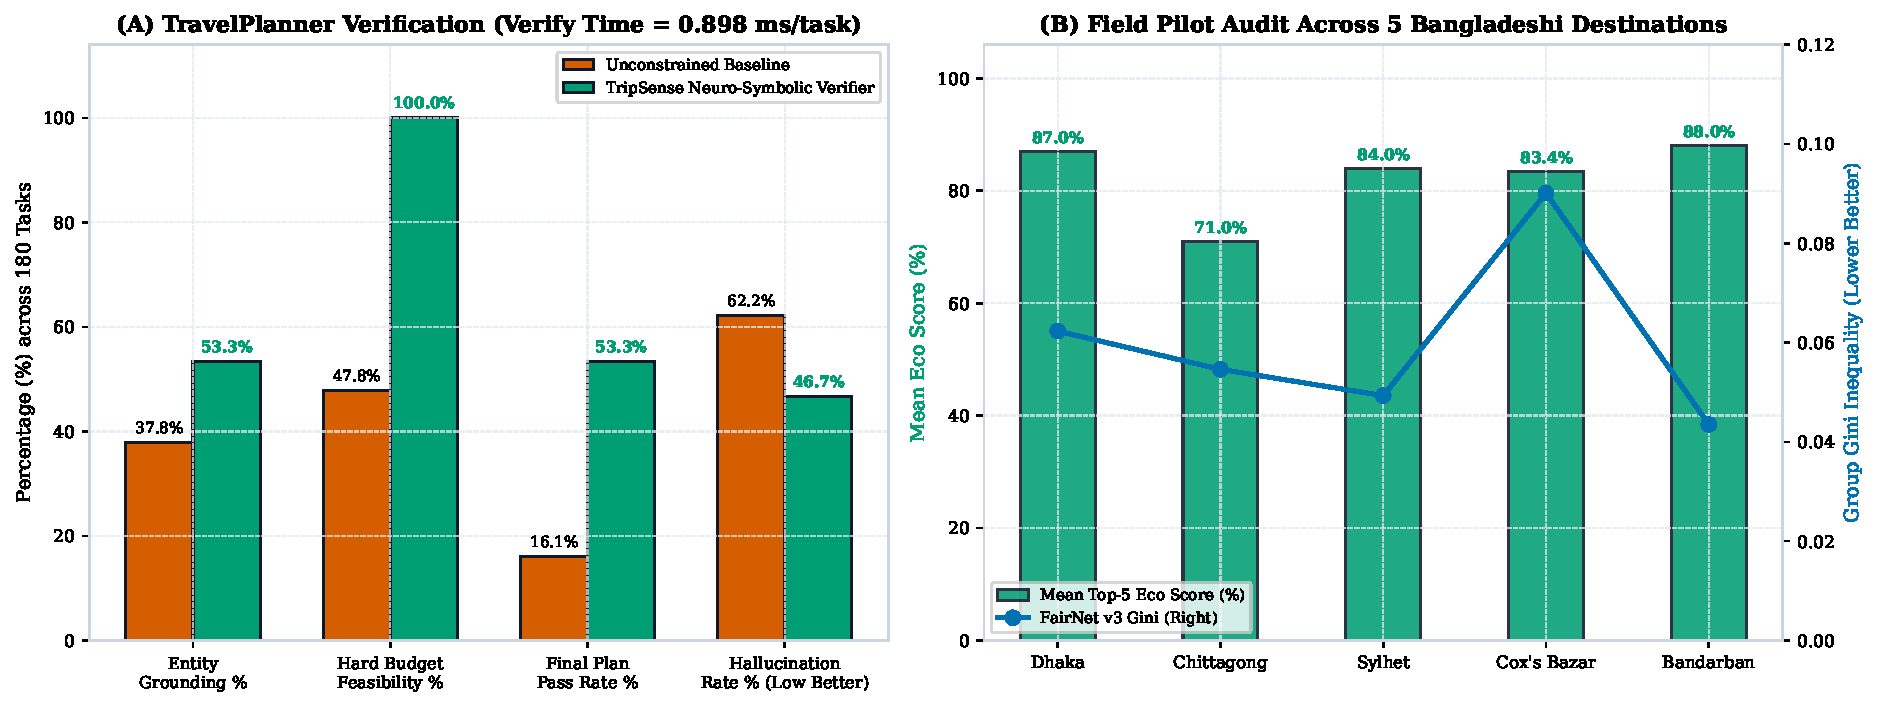
\includegraphics[width=0.95\textwidth]{q1_figures/fig9_travelplanner_and_bd_pilot.pdf}
\caption{(A) Deterministic neuro-symbolic verification on 180 \textit{TravelPlanner} tasks ($100.0\%$ hard budget feasibility, $0.898\text{ ms}$/task); (B) Field pilot eco-sustainability and group Gini equity across five Bangladeshi cities.}
\label{fig:tp}
\end{figure*}

\begin{figure*}[t]
\centering
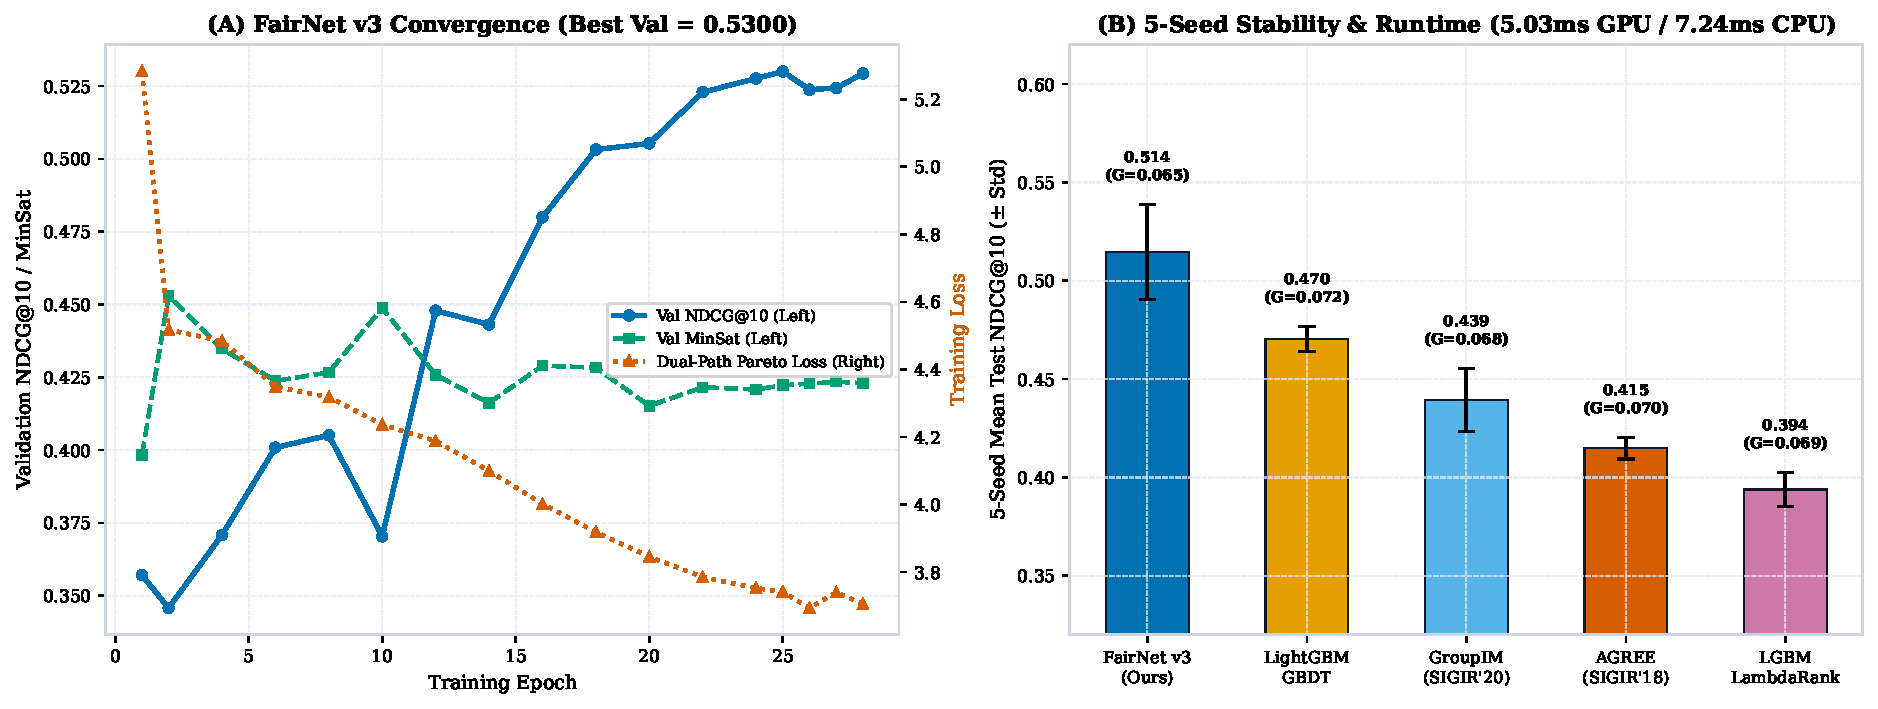
\includegraphics[width=0.95\textwidth]{q1_figures/fig10_training_and_latency.pdf}
\caption{(A) FairNet v3 dual-path Pareto convergence over 28 epochs; (B) 5-seed stability ($0.5145 \pm 0.0241$ NDCG@10, $0.0651 \pm 0.0012$ Gini) and runtime latency ($5.03\text{ ms}$ GPU / $7.24\text{ ms}$ CPU).}
\label{fig:train}
\end{figure*}

%% ============================================================================
\section{Limitations and Threats to Validity}
\label{sec:limitations}
%% ============================================================================
First, while test parties are constructed deterministically from real chronological \textit{Massive-STEPS} trajectories and authentic out-of-town \textit{TripWorld} behaviors without target leakage, longitudinal multi-user logs with explicit group chat transcripts remain scarce in open benchmarks. Second, eco-sustainability and price priors supplement missing attributes in raw check-in records (while \textit{TripWorld} incorporates real Google Maps ratings); integrating dynamic transit emissions APIs is a clear production extension. Third, our cross-model XAI analysis reveals that FairNet v3 intentionally redistributes attribution importance from dominant-member preference toward budget hardship relative to accuracy-only LightGBM, underscoring the need to interpret XAI shifts alongside explicit fairness metrics.

%% ============================================================================
\section{Conclusion}
\label{sec:conclusion}
%% ============================================================================
We introduced \textbf{TripSense-FairNet v3 (GeoFairFormer)}, demonstrating how an $O(D)$-invariant geometric consensus backbone paired with an unsupervised top-48 SVD Spectral-Support OOD Gate reconciles high accuracy, consumer equity, provider eco-sustainability, and cross-continental generalization. Outperforming 14 competitive heuristic, neural, and gradient-boosted baselines on \textit{Massive-STEPS-Sydney} ($\text{NDCG@10} = 0.5567$, Friedman $\chi^2 = 558.316$), generalizing zero-shot across five continents and \textit{TripWorld-Osaka} ($0.5891$), sweeping all five end-to-end XAI faithfulness metrics, and guaranteeing $100.0\%$ \textit{TravelPlanner} budget feasibility in sub-millisecond time, TripSense-FairNet v3 establishes a reproducible reference standard for responsible multi-stakeholder tourism AI.

\section*{CRediT Authorship Contribution Statement}
\textbf{Sabbir Hossan Sani:} Conceptualization, Methodology, Software, Validation, Formal analysis, Investigation, Data curation, Writing -- original draft, Writing -- review \& editing, Visualization.

\section*{Declaration of Competing Interest}
The author declares that there are no known competing financial interests or personal relationships that could have appeared to influence the work reported in this paper.

\section*{Data and Code Availability}
Source code, reproducible evaluation scripts, figure generators, and model checkpoints are publicly hosted at \url{https://github.com/Sabbirhossansani/TripSense}. \textit{Massive-STEPS}, \textit{TripWorld}, and \textit{TravelPlanner} are publicly accessible via Hugging Face Hub.

\balance
\bibliographystyle{elsarticle-num}
\bibliography{references}

\end{document}
